\chapter{INTRODUCTION}
\label{chap:intro}

\section{Background}
The study of rotating cantilever beams has been around since the early days of aviation. For example, the fundamental study in this area was published in 1922 by Southwell and Gough, Ref.~\cite{southwell1922free}. The dynamics of airscrew blades were studied and an error calculation was provided to bound the error of the approximation. The work is important because it acknowledged that rotation speed affects the stiffness of a beam and then studied how the rotation speed changed the frequencies of the natural modes of vibration. The stiffening of the beam due to rotation increases the natural frequencies and this work provided an upper bound to the correction of the frequencies based upon rotation speed. In 1973, Belytschko and Hsieh studied the efficiency of convected coordinates on finite element approximation techniques Ref~\cite{belytschko1973non}. Hoa studied finite element approximation to blades with tip mass and varied setting angle in 1979, Ref.~\cite{hoa1979vibration}. In 1980, Hale and Meirovitch studied a method of finite element analysis in which fewer degrees of freedom can be used as the system is reduced to substructures, Ref~\cite{hale1980general}. Christensen and Lee studied nonlinear finite element analysis and time integration of rigid bodies undergoing large translations and rotations Ref.~\cite{christensen1986nonlinear}. In 1988, Yokoyama explored the vibration of rotating cantilever beams using the full Timoshenko beam theory approach to the finite element model in Ref.~\cite{yokoyama1988free}. Lee and Kuo studied the effects of twist, taper, setting angle and hub connection elasticity on the natural frequencies of the rotating cantilever beam in their 1992 work Ref.~\cite{lee1992bending}. The work by Yoo, Ryan and Scott in 1995 greatly improved the accuracy of the numerical results for elastic beams by creating a transformation to a stretch coordinate frame for one of the displacement directions and coupling the stretch to the in plane and out of plane displacements, Ref.~\cite{yoo1995dynamics}. In 1998, Yoo and Shin studied the effects of gyroscopic coupling on rotating beams in Ref.~\cite{yoo1998shin}. Yoo, Kwak and Chung as well as Yoo, Park and Park studied pre-twisted beams using the stretch coordinate frame transformation in 2001, Refs.~\cite{yoo2001twist},~\cite{yoo2001parkpark}. The 2008 Ozgumus and Kaya study investigated doubly tapered beams in Ref.~\cite{ozgumus2008flapwise} and the 2011 study by Zhu explored pretwisted rotating Timoshenko beams using finite element analysis in Ref.~\cite{zhu2011vibrations}. As recently as 2013, Kim, Yoo and Chung have studied rotating cantilever beams in Ref.~\cite{kim2013dynamic}. In short, although rotating beams have been studied for a century, there is ongoing work in the field to improve the accuracy and reliability of finite element analysis techniques centered on accounting for more complex effects and geometries of the beams.

\section{Organization}
This study is organized as follows. First, the equations of motion are developed from first principles of physics in Chapter~\ref{chap:eom}. More specifically, Section~\ref{sec:energy_eqns} develops the energy equations, while Section~\ref{sec:variations} uses variational approximation to develop the equations of motion and Section~\ref{sec:discretizing} describes the discretization process.

Chapter~\ref{ch:results} provides numerical results and analyzes the results. Section~\ref{sec:validation} validates the model against previous results and Section~\ref{sec:exp} develops the experimental design. Section~\ref{sec:results} provides the experimental results and analysis.

Finally, Chapter~\ref{ch:conclusion} summarizes the work and describes what challenges lie ahead.

\chapter{EQUATIONS OF MOTION}
\label{chap:eom}
The equations of motion of the rotating cantilever beam system are developed through the principles of variational approximation as covered in Appendix \ref{app:variations}. We begin by describing the energy equations of the system, then apply variational approximation to formulate the approximating form and apply the discretizing interpolation for a single element two-node system. Finally, the system is expanded to $N$-dimensional form, and the system matrices are formulated. 

\section{Energy Equations}
\label{sec:energy_eqns}
The energy equations consist of kinetic energy, denoted by $T$, and potential energy, denoted by $V$. These are precisely the quantities discussed in Appendix \ref{app:variations}. In this case, the beam is discretized as a coupled mass-spring system. The coupling is determined by the equations of motion resulting from integration, simplification and interpolation. The system that shall be considered is the system discussed in Ref.~\cite{chung2002dynamic}. In this system, it is assumed that the beam is long compared to its height and thickness, so that shear deformations may be neglected. 

The beam is affixed to a central hub which is rotated at a frequency $\Omega$. The direction which is in-plane with the rotations and along the length of the beam is referred herein as the axial direction, labeled $u$. The direction which is in-plane with rotations and orthogonal to the $u$ direction is referred to as the chord-wise direction, and is labeled $v$. The out-of-plane direction, which is orthogonal to both $u$ and $v$, is referred to as the flap-wise direction and is labeled $w$ (see Fig.~\ref{fig:canti_diag}).

\begin{figure}[ht!]
\label{fig:canti_diag}
\caption[Cantilever beam with rotation about a central hub.]{Cantilever beam with rotation about a central hub. \protect\bibentry{chung2002dynamic}.}
\centering
\includegraphics[width=0.65\textwidth]{images/chung_yoo_cantilever_beam.pdf}
\end{figure}

\subsection{Stretch Coordinate Frame}
\label{subsec:stretch}
Any displacement will cause elongation or shortening of the beam, which shall be named stretch and assigned the variable $s$. The stretch is affected by all displacement coordinates, $u,v,w$. Consequently, accounting for stretch from displacements in the Cartesian reference frame becomes unwieldy to maintain. In order to remedy this, it is necessary to create a coordinate relation between the displacements and the stretch. This section follows closely to the work done in Ref.~\cite{lima2012thesis}.

Consider the diagram given by Fig.~\ref{fig:stretch_coord_lima}. In this diagram, the $u$ direction has been replaced by a dummy variable $\eta$ in order to prevent confusion during the derivation of the stretch term, $s$. 

\begin{figure}[ht!]
\caption[Stretch coordinate relation diagram.]{Stretch coordinate relation diagram. \protect\bibentry{lima2012thesis}}
\label{fig:stretch_coord_lima}
\centering
\includegraphics[width=0.65\textwidth]{images/stretch_coords.eps}
\end{figure}

\noindent From Pythagoras, we have the length of the hypotenuse of the infinitesimal displacements $\text d\eta, \text dv, \text dw$ given as
\begin{equation}
\text dS = \sqrt{(\text d\eta)^2+(\text dv)^2+(\text dw)^2},
\label{eq:pythag.basic}
\end{equation}
and integrating both sides of Eq.~(\ref{eq:pythag.basic}) yields
\begin{equation}
S = \int_0^{x+u} \sqrt{(\text d\eta)^2+(\text dv)^2+(\text dw)^2},
\label{eq:arclength.a}
\end{equation}
which is known as the arclength integral in $\mathbb R^3$. Notice that the integration is done with respect to $\eta$, and varies over 0 to $x+u$ as in the diagram. \emph{Note:} the arclength $S$ is not equivalent to stretch $s$. This integral is complicated to compute in this form, so a change of variables is introduced. Let
\begin{equation}
\phi = \eta - u
\end{equation}
so that
\begin{equation}
\text d\eta = \text d\phi + \text du.
\label{eq:pythag.subs.vars}
\end{equation}
The integration limits are converted by considering that at the center of the rotation, the displacement will be zero in all directions, so that stretch is zero. For the upper limit, consider that $\eta = u+x$ so that $\phi = x$. 

Substituting Eq.~(\ref{eq:pythag.subs.vars}) into Eq.~(\ref{eq:pythag.basic}) yields
\begin{equation}
\text dS = \sqrt{(\text d\phi + \text du)^2+(\text dv)^2+(\text dw)^2}.
\end{equation} 
By the chain rule, this can be rewritten as
\begin{equation}
\text dS = \left[\left(\text d\phi + \frac{\partial u}{\partial\phi}\text d\phi\right)^2+\left(\frac{\partial v}{\partial\phi}\text d\phi\right)^2+\left(\frac{\partial w}{\partial\phi}\text d\phi\right)^2\right]^{1/2}.
\end{equation}
Factoring out $\text d\phi$, replacing the integration limits, and substitution into Eq.~(\ref{eq:arclength.a}) yields
\begin{equation}
S = \int_0^x \left[\left(1 + \frac{\partial u}{\partial\phi}\right)^2+\left(\frac{\partial v}{\partial\phi}\right)^2+\left(\frac{\partial w}{\partial\phi}\right)^2\right]^{1/2}\text{ d}\phi.
\label{eq:arclength.b}
\end{equation}
The first term in Eq.~(\ref{eq:arclength.b}) is expanded as
\begin{equation}
\left(1 + \frac{\partial u}{\partial\phi}\right)^2 = 1+2\frac{\partial u}{\partial\phi}+\left(\frac{\partial u}{\partial\phi}\right)^2,
\label{eq:arclength.expansion}
\end{equation}
and considering the infinitesimals
\begin{equation}
\label{eq:arclength.u.assump}
1+2\frac{\partial u}{\partial\phi} \gg \left(\frac{\partial u}{\partial\phi}\right)^2,
\end{equation}
we approximate Eq.~(\ref{eq:arclength.expansion}) as
\begin{equation}
\left(1 + \frac{\partial u}{\partial\phi}\right)^2 \approx 1+2\frac{\partial u}{\partial\phi}.
\label{eq:arclength.u.approx}
\end{equation}
Let
\begin{equation}
f(y) = (1+y)^{1/2},
\end{equation}
with McLaurin expansion
\begin{eqnarray}
f(y) &=& f(0)+f'(0)y+\frac{1}{2}f''(0)y^2+\cdots{\vrule width 0in depth .1in}\nonumber \\
&=& (1+0)^{1/2}+\frac{1}{2}(1+0)^{-1/2}y-\frac{1}{4}(1+0)^{-3/2}y^2+\cdots{\vrule width 0in depth .1in}\nonumber \\
&=& 1+\frac{y}{2}-\frac{y^2}{4}+\cdots,
\end{eqnarray}
and assuming small variations so that $y^2\ll y$, we approximate $f$ near 0 by
\begin{equation}
f(y) \approx 1+\frac{y}{2}.
\label{eq:f_func.approx}
\end{equation}
Plugging Eq.~(\ref{eq:arclength.u.approx}) in to Eq.~(\ref{eq:arclength.b}) yields
\begin{equation}
S = \int_0^x \left[1+2\frac{\partial u}{\partial\phi}+\left(\frac{\partial v}{\partial\phi}\right)^2+\left(\frac{\partial w}{\partial\phi}\right)^2\right]^{1/2} \text{ d}\phi.
\end{equation}
Observe that this can be rewritten as 
\begin{equation}
S = \int_0^x \left[1+\left\lbrace 2\frac{\partial u}{\partial\phi}+\left(\frac{\partial v}{\partial\phi}\right)^2+\left(\frac{\partial w}{\partial\phi}\right)^2\right\rbrace\right]^{1/2} \text d\phi,
\label{eq:arclength.grouped}
\end{equation}
and for 
\begin{equation}
y = 2\frac{\partial u}{\partial\phi}+\left(\frac{\partial v}{\partial\phi}\right)^2+\left(\frac{\partial w}{\partial\phi}\right)^2,
\end{equation}
the approximation in Eq.~(\ref{eq:f_func.approx}) may be applied to Eq.~(\ref{eq:arclength.grouped}) so that arclength may be written as
\begin{equation}
S = \int_0^x 1+\frac{1}{2}\left[ 2\frac{\partial u}{\partial\phi}+\left(\frac{\partial v}{\partial\phi}\right)^2+\left(\frac{\partial w}{\partial\phi}\right)^2 \right]\text{ d}\phi.
\end{equation}
Distribution of the constant $1/2$ and integration over the first two terms yields
\begin{equation}
S = x + u + \frac{1}{2}\int_0^x\left(\frac{\partial v}{\partial\phi}\right)^2\text{ d}\phi+\frac{1}{2}\int_0^x\left(\frac{\partial w}{\partial\phi}\right)^2\text{ d}\phi.
\end{equation}
We now define the stretch term $s$ in relation to the arclength $S$ by
\begin{equation}
S = x+s,
\end{equation}
so that stretch can be written as
\begin{equation}
s = u + \frac{1}{2}\int_0^x\left(\frac{\partial v}{\partial\phi}\right)^2\text{ d}\phi+\frac{1}{2}\int_0^x\left(\frac{\partial w}{\partial\phi}\right)^2\text{ d}\phi.
\end{equation}
For ease of notation, let
\begin{eqnarray}
h_v &\equiv& \frac{1}{2}\int_0^x\left(\frac{\partial v}{\partial\phi}\right)^2\text{ d}\phi,{\vrule width 0in depth .1in}\\
h_w &\equiv& \frac{1}{2}\int_0^x\left(\frac{\partial w}{\partial\phi}\right)^2\text{ d}\phi,
\end{eqnarray}
so that 
\begin{equation}
s = u+h_v+h_w.
\label{eq:stretch.full}
\end{equation}
The temporal rate of change of stretch can thus be expressed as 
\begin{equation}
\dot s = \dot u + \dot h_v+\dot h_w,
\label{eq:stretch.full.dt}
\end{equation}
where the chain rule yields
\begin{eqnarray}
\dot h_v &=& \int_0^x\frac{\partial v}{\partial\phi}\frac{\partial \dot v}{\partial\eta}\text{ d}\phi,{\vrule width 0in depth .1in}\\
\dot h_w &=& \int_0^x\frac{\partial w}{\partial\phi}\frac{\partial \dot w}{\partial\eta}\text{ d}\phi.
\end{eqnarray}

With the book-keeping surrounding stretch completed, it is now possible to obtain the equations of motion. Note, however, that there were many assumptions that will require the numerics to include a sufficiently fine grid in both time and space such that the assumptions are valid. A discussion of what ``sufficiently fine'' pertains to is given in Section~\ref{sec:discretizing}.

\subsection{Kinetic Energy}
The system's kinetic energy is given by the classical scalar kinetic energy formulation
\begin{equation}
T = \frac{1}{2}m\vec{\textbf{v}}^2.
\label{eq:kin.scalar}
\end{equation}

\noindent The generalized integral representation of this equation is given by

\begin{equation}
T = \frac{1}{2}\int_{0}^{L}\rho A \vec{\textbf{v}}\cdot\vec{\textbf{v}}\text{ d}x,
\label{eq:kin.int.full}
\end{equation}
where $L$ is the length of the cantilever beam, $\rho$ and $A$ are the point density and cross section area, respectively. The units for $\rho$ are $\frac{\text{kg}}{\text{m}^3}$, and $A$ is $\text{m}^2$, and since Eq.~(\ref{eq:kin.int.full}) integrates upon a singular axis, we recover mass along a single axis by the product $\rho A$ at each point along the beam.

If density and cross section are uniform along the entire beam, Eq.~(\ref{eq:kin.int.full}) can be written as

\begin{equation}
T = \frac{1}{2}\rho A\int_{0}^{L}\vec{\textbf{v}}\cdot\vec{\textbf{v}}\text{ d}x,
\label{eq:kin.int.iso}
\end{equation}
where, for each point on the beam, Eq.~(\ref{eq:kin.int.iso}) is precisely the same as Eq.~(\ref{eq:kin.scalar}). From the rotation, and deformation corresponding to bending, the velocity at the point $P$ is

\begin{equation}
\vec{\textbf{v}}_p = (\dot u-\Omega v)\textbf{i}+[\dot v+\Omega(a+x+u)]\textbf{j}+ \dot w\textbf{k}.
\label{eq:vel.vec}
\end{equation}
Rotation induces angular momentum, and allowing for stretch along the axial direction yields that the momentum from the rotational speed $\Omega$ is calculated by

\begin{equation}
L = \Omega\cdot(a+x+u) A\rho,
\label{eq:ang.mom}
\end{equation}
where $(a+x)$ is the point position along the axial direction when the system is at rest and $u$ is the displacement along the axial direction when the system is rotating at frequency $\Omega$.

The corresponding direction of rotation is the same direction as $v$, so that the chord-wise component of velocity is increased by this momentum. Assuming conserved momentum, a change in the chord-wise direction must result in a change in the axial direction. Then an increase in momentum in the chord-wise direction must result in a decrease in momentum in the axial direction, so that the $-\Omega v$ term in Eq.~(\ref{eq:vel.vec}) is required.  The flap-wise direction is unaffected, and it is not present in Eq.~(\ref{eq:ang.mom}). The assumption of conserved momentum is valid since the system achieves stability; otherwise, the momentum would grow rapidly and the beam would break. 

Plugging Eq.~(\ref{eq:vel.vec}) into Eq.~(\ref{eq:kin.int.iso}) finally yields the following expression for the kinetic energy:
\begin{align}
T &= \frac{1}{2}\rho A\int_{0}^{L}\left\langle(\dot u-\Omega v)\textbf{i}+[\dot v+\Omega(a+x+u)]\textbf{j}+ \dot w\textbf{k}\right\rangle^2\text{ d}x, \\
  &= \frac{1}{2}\rho A\int_{0}^{L} (\dot u-\Omega v)^2+[\dot v+\Omega(a+x+u)]^2+\dot w^2\text{ d}x.
  \label{eq:kin.final}
\end{align}

\subsection{Potential Energy}

The potential energy of the system is taken to be strain energy; the effects of gravity are considered small relative to the other forces. This is because when deformed, the beam will try to restore itself to its original shape; the restoring force can be thought of as stored energy, and typically this is called strain energy. This assumption is taken because of the properties of the material that shall be considered, typically metals such as steel and aluminum, which do not permanently deform but restore to their original shape after deformation.

\subsubsection{Strain Energy}
We start by incorporating the results from Appendix~\ref{app:strain}. By considering an applied force to the beam and applying Eq.~(\ref{eq:stress.force}) to Eq.~(\ref{eq:strain.energy.final}), we rewrite the total strain energy as
\begin{equation}
U = \int_0^L\int_A\frac{1}{2E}\left(\frac{F}{A}\right)^2\text{ d}A\text{ d}x,
\end{equation}
where $F$ is the applied force and $E$ is the material constant known as Young's modulus, then integrate over the area $A$ to find
\begin{equation}
U = \int_0^L\frac{F^2}{2EA}\text{ d}x.
\end{equation}
The axial stress resultant from stretch can be expressed by considering the stress-strain relationship in Eq.~(\ref{eq:strain.hooke}), and applying the strain definition from Eq.~(\ref{eq:strain.oned}), we write
\begin{equation}
\sigma = E\frac{\partial s}{\partial x}
\end{equation} 
thus
\begin{equation}
U_{\text{stretch}} = \int_0^L\frac{EA}{2}\left(\frac{\partial s}{\partial x}\right)^2\text{ d}x.
\end{equation}

\noindent The strain induced by bending is given by
\begin{equation}
\varepsilon = -\frac{y}{\rho},
\label{eq:strain.bend.basic}
\end{equation}
where $y$ is the distance from the neutral plane. For axisymmetric geometries, maximum strain occurs at the boundary (\emph{i.e.} for a cylinder, the radius). $\rho$ is given as the radius of curvature; that is, the radius of the osculating circle that best fits the curvature of the bend. The radius of curvature in 2D orthogonal (or cartesian) coordinates is expressed as the arclength of the path traveling along the rod.  The arclength integral is computed to be 
\begin{equation}
\rho = \left|\frac{(1+{y'}^2)^{3/2}}{y''}\right|.
\end{equation}
Here, $y'$ is the derivative of $y$ with respect to $x$. We now assume that the bending is small so that $y'\ll1$ and approximate the radius of curvature to be
\begin{equation}
\rho = \left(\frac{\text d^2y}{\text dx^2}\right)^{-1}.
\label{eq:radius.curvature}
\end{equation}
This assumption is valid for the metallic alloys we are considering as a result of material properties. Additionally, we are in a coordinate frame in which we will consider the directions $u,v,w$ with respect to $x$.

Substituting Eq.~(\ref{eq:radius.curvature}) into Eq.~(\ref{eq:strain.bend.basic}), and adjusting into the flap-wise coordinate frame yields
\begin{equation}
\varepsilon = -y\left(\frac{\partial^2v}{\partial x^2}\right),
\end{equation}
and using the stress-strain relationship given in Eq.~(\ref{eq:strain.hooke}), we find
\begin{equation}
\sigma = -Ey\left(\frac{\partial^2v}{\partial x^2}\right).
\label{eq:stress.bending.early}
\end{equation}
The bending moment, $M$, is defined to be 
\begin{equation}
M = -\int_Ay\sigma \text{ d}A = \int_AEy^2\left(\frac{\partial^2v}{\partial x^2}\right)\text{ d}A.
\end{equation}
For each subsection along $x$, both $E$ and $\frac{\partial^2v}{\partial x^2}$ are considered constant with respect to the area, and we write the integral as
\begin{equation}
M = E\left(\frac{\partial^2v}{\partial x^2}\right)\int_Ay^2\text{ d}A.
\label{eq:moment.inertia}
\end{equation}
The quantity resulting from the area integral is known as the \emph{moment of inertia}, and in this case it is the second moment about $z$, written as
\begin{equation}
I_{zz} = \int_Ay^2\text{ d}A.
\end{equation}
With this simplification, we write the bending moment as
\begin{equation}
M_z = EI_{zz}\left(\frac{\partial^2v}{\partial x^2}\right).
\end{equation}
Upon substitution for $\frac{\partial^2v}{\partial x^2}$, we may rewrite Eq.~(\ref{eq:stress.bending.early}) as
\begin{equation}
\sigma = \frac{M_zy}{I_{zz}}.
\label{eq:stress.bending.full}
\end{equation}
Plugging this stress into the strain integral from Eq.~(\ref{eq:strain.energy.final}) we have
\begin{equation}
U_{\text{bending}} = \int_0^L\int_A\frac{1}{2}\frac{\sigma^2}{E}\text{ d}A\text{ d}x = \int_0^L\int_A\frac{1}{2E}\left(\frac{M_zy}{I_{zz}}\right)^2\text{ d}A\text{ d}x.
\end{equation}
Distributing the power, we use the principle from Eq.~(\ref{eq:moment.inertia}) to pull out the terms not involving $y$, and integrating over the cross-section area cancels one moment of inertia term $I_{zz}$, which yields
\begin{equation}
U_{\text{bending}} = \int_0^L\frac{M_z^2}{2EI_{zz}}\text{ d}x,
\end{equation}
and substituting for $M_z$ yields
\begin{equation}
U_{\text{bending}} = \int_0^L\frac{EI_{zz}}{2}\left(\frac{\partial^2 v}{\partial x^2}\right)^2\text{ d}x.
\label{eq:strain.bending.final}
\end{equation}

This term holds for bending in two directions, flap-wise ($v$) and chord-wise ($w$). In the case of chord-wise bending, the bending moment is written as $M_y$, the moment of inertia is $I_{yy}$, and the inverse radius of curvature is given as $\frac{\partial^2w}{\partial x^2}$. Otherwise, the formulation is precisely the same.

Finally, the full strain energy equation is a combination of the above discussed terms, given as
\begin{equation}
U = \int_0^L\frac{E}{2}\left[I_{zz}\left(\frac{\partial^2 v}{\partial x^2}\right)^2+I_{yy}\left(\frac{\partial^2 w}{\partial x^2}\right)^2+A\left(\frac{\partial s}{\partial x}\right)^2\right]\text{ d}x.
\label{eq:strain.final.chooyung}
\end{equation}

\section{Applying Variational Approximation}
\label{sec:variations}
Now that the kinetic and potential energy equations have been determined, the principles of variational approximation may be used to approximate the equations of motion. We begin by writing the Lagrangian of the system, then rearranging the system by way of integration by parts to develop the Euler-Lagrange equations for the system. The non-vanishing terms that are not included in the Euler-Lagrange formulation are used to formulate approximation functions which both satisfy the boundary conditions and vanish as required to permit the use of variational approximation. Additionally, the properties of the physical system are considered when choosing the class of test functions which might be appropriate.

\subsection{Developing the Euler-Lagrange Equations}
The Lagrangian is given by 
\begin{equation}
L = T-V = T-U.
\end{equation}
Applying variations as in Appendix~\ref{app:variations}, we have the functional 
\begin{equation}
J = \int_{t_0}^{t_1}L\text{ d}t
\end{equation}
to be minimized as
\begin{equation}
\delta J = \delta\int_{t_0}^{t_1}L\text{ d}t.
\end{equation}
By the linearity of $\delta$ we may move the variation inside the integral as
\begin{equation}
\delta J = \int_{t_0}^{t_1}\delta L\text{ d}t = \int_{t_0}^{t_1}\delta (T-U)\text{ d}t = \int_{t_0}^{t_1}\delta T - \delta U\text{ d}t.
\end{equation}

For $T$ and $U$, each has a spatial integral. We define the subfunctions $\hat T$ and $\hat U$ as
\begin{eqnarray}
T = \int_0^L \hat T \text{ d}x, \\
U = \int_0^L \hat U \text{ d}x,
\end{eqnarray}
and write
\begin{equation}
\delta J = \int_{t_0}^{t_1}\int_{0}^{L}\delta\hat T - \delta\hat U\text{ d}x\text{ d}t.
\end{equation}
The chain rule for the variational operator requires that each independent variable of the function under variation is considered. For the kinetic energy, we have that
\begin{equation}
\hat T = \hat T(u,\dot u,v,\dot v,w,\dot w),
\end{equation}
which yields 
\begin{equation}
\delta \hat T = \sum_{p_i}\frac{\partial \hat T}{\partial p_i}\delta p_i+\frac{\partial \hat T}{\partial \dot{p_i}}\delta \dot{p_i},\qquad p_i\in\{u,v,w\}.
\end{equation}
Note that there explicitly is not a function $w$ in $\hat T$, but including this term for ease of notation is harmless since $\frac{\partial\hat T}{\partial w}=0$. For the potential energy function, we have that
\begin{equation}
\hat U = \hat U(s_x,v_{xx},w_{xx}),
\end{equation}
which yields 
\begin{equation}
\delta \hat U = \sum_{q_j}\frac{\partial \hat U}{\partial q_j}\delta q_j,\qquad q_j\in\{s_x,v_{xx},w_{xx}\}.
\end{equation}
In order to properly formulate the Lagrangian of the system, we must transform these coordinates so that terms are given in $\delta s,\delta v,\delta w$. Integration by parts shall be employed in various ways in order to derive the Lagrangian in this form.

We first introduce a tool to transform products by way of integration by parts. The assumptions are strict and specific, but are well suited for problems in this domain, since they always apply to cantilever beams.

\begin{lemma}
Let $f$ be an integrable function in the domain $[0,L]$ and define $F = \int f(x)\text{ d}x$ on $[0,L]$. If $F(0) = f(L) = 0$, then given the integrable function $g$,
\begin{equation}
I = \int_0^L\left(\int_0^xg(\xi)\text{ d}\xi\right)f(x)\text{ d}x = \int_0^L\left(\int_L^xf(\xi)\text{ d}\xi\right)g(x)\text{ d}x.
\end{equation}
\label{lem:switch.integrals}
\end{lemma}
\begin{proof}
We perform integration by parts as follows. Let
\[\alpha = \int_0^xg(\xi)\text{ d}\xi.\]
Then
\[\text{d}\alpha = g(x)\text{ d}x\]
by the Fundamental Theorem of Calculus. Let
\[\text{d}\beta = f(x)\text{ d}x.\]
Then
\[\beta = F(x).\]
Applying the integration by parts formula, we have
\begin{equation*}
\begin{array}{rcll}
I &=&  \left.\int_0^xg(\xi)\text{ d}\xi F(x)\right|_0^L - \int_0^LF(x)g(x)\text{ d}x & \\
  &=&  \int_0^Lg(x)\text{ d}xF(L) - \int_0^LF(x)g(x)\text{ d}x &\text{(since $F(0)=0$)} \\
  &=&  \int_0^LF(L)g(x)\text{ d}x - \int_0^LF(x)g(x)\text{ d}x &\text{(since $F(L)$ is constant)} \\
  &=&  \int_0^L[F(L)-F(x)]g(x)\text{ d}x &\text{(by linearity)} \\
  &=&  \int_0^L\left(\int_L^xf(\xi)\text{ d}\xi\right)g(x)\text{ d}x &\text{(by definition of $F$)} \\
\end{array}
\end{equation*}
\end{proof}

Since time $t$ and space $x$ are independent of each other, the iterated integrals may be switched, and we may write the variation on $\hat T$ as
\begin{equation}
\int_{t_0}^{t_1}\int_0^L\delta\hat T\text{ d}x\text{ d}t = \int_0^L\int_{t_0}^{t_1}\delta\hat T\text{ d}t\text{ d}x.
\end{equation}
The term for $q_i=u$ has special properties and we shall consider those properties later; we first analyze $q_i\in\{v,w\}$. The $\dot q_i$ term is integrated by using integration by parts. This is accomplished by using the time integral; the spatial integral shall be excluded for brevity.
First, write out the full variation on the kinetic energy:
\begin{equation}
\int_{t_0}^{t_1}\delta\hat T(\dot q_i,q_i)\text{ d}t = \int_{t_0}^{t_1}\frac{\partial\hat T}{\partial \dot q_i}\delta \dot q_i\text{ d}t+\int_{t_0}^{t_1}\frac{\partial\hat T}{\partial q_i}\delta q_i\text{ d}t.
\label{eq:kin.variation}
\end{equation}
Then, consider the first integral on the right hand side, and let
\begin{equation}
\alpha = \frac{\partial\hat T}{\partial \dot q_i},
\end{equation}
then
\begin{equation}
\text{ d}\alpha = \frac{\text d}{\text dt}\left(\frac{\partial\hat T}{\partial \dot q_i}\right)\text{ d}t.
\end{equation}
Next, let
\begin{equation}
\text{d}\beta = \delta \dot q_i\text{ d}t,
\end{equation}
then
\begin{equation}
\beta = \int \frac{\text d}{\text dt}(\delta q_i)\text{ d}t = \delta q_i.
\end{equation}
Finally, we may write the first integral as
\begin{equation}
\int_{t_0}^{t_1}\frac{\partial\hat T}{\partial \dot q_i}\delta \dot q_i\text{ d}t = \left.\frac{\partial\hat T}{\partial \dot q_i}\delta q_i\right |_{t_0}^{t_1}-\int_{t_0}^{t_1}\frac{\text d}{\text dt}\left(\frac{\partial\hat T}{\partial \dot q_i}\right)\delta q_i\text{ d}t.
\end{equation}
The variational approximation requires that
\begin{equation}
\left.\frac{\partial\hat T}{\partial \dot q_i}\delta q_i\right |_{t_0}^{t_1} = 0,\quad\forall i,
\end{equation}
thus the first integral is given by
\begin{equation}
\int_{t_0}^{t_1}\frac{\partial\hat T}{\partial \dot q_i}\delta \dot q_i\text{ d}t = -\int_{t_0}^{t_1}\frac{\text d}{\text dt}\left(\frac{\partial\hat T}{\partial \dot q_i}\right)\delta q_i\text{ d}t.
\label{eq:kin.variation.byparts}
\end{equation}
Substitution of Eq.~(\ref{eq:kin.variation.byparts}) into Eq.~(\ref{eq:kin.variation}) yields
\begin{equation}
\int_{t_0}^{t_1}\delta\hat T(\dot q_i,q_i)\text{ d}t = \int_{t_0}^{t_1}\left\lbrace-\frac{\text d}{\text dt}\left[\frac{\partial\hat T}{\partial \dot q_i}\right]+\frac{\partial\hat T}{\partial q_i}\right\rbrace\delta q_i\text{ d}t.
\end{equation}
We now reintroduce the spatial integral and switch the order of integration so that $\hat T$ and $\hat U$ are integrating in the same order, which yields
\begin{equation}
\int_{t_0}^{t_1}\int_0^L\delta\hat T(\dot q_i,q_i)\text{ d}x\text{ d}t = \int_{t_0}^{t_1}\int_0^L\left\lbrace-\frac{\text d}{\text dt}\left[\frac{\partial\hat T}{\partial \dot q_i}\right]+\frac{\partial\hat T}{\partial q_i}\right\rbrace\delta q_i\text{ d}x\text{ d}t.
\end{equation}

We now continue the process for strain energy. The strain energy $U$ yields differing variation fields which must be converted to be in the $q_i$ form. The dynamic expressions in $U$ are given in Eq.~(\ref{eq:strain.final.chooyung}) as $v_{xx}$, $w_{xx}$, and $s_x$. The generalized coordinates are $q_{xx_i}$ and $q_{x_i}$, where the subscript $x$ represents the derivative with respect to $x$ and the subscript $i$ represents the $i$-th direction.

The chain rule applied to the strain term $U$ is given by
\begin{equation}
\delta U(q_{xx_i},q_{x_i}) = \frac{\partial U}{\partial q_{xx_i}}\delta q_{xx_i}+\frac{\partial U}{\partial q_{x_i}}\delta q_{x_i}.
\end{equation}
Once again, we aim to modify this expression so that the terms on the right are given as variations of $q_i$.
The full variation of the strain energy is given as
\begin{equation}
\int_{t_0}^{t_1}\delta U(q_{xx_i},q_{x_i})\text{ d}t = \int_{t_0}^{t_1}\frac{\partial U}{\partial q_{xx_i}}\delta q_{xx_i}\text{ d}t+\int_{t_0}^{t_1}\frac{\partial U}{\partial q_{x_i}}\delta q_{x_i}\text{ d}t.
\end{equation}
We now rewrite $U$ as
\begin{equation}
U = \int_0^L \hat{U}\text{ d}x,
\end{equation}
so that
\begin{equation}
\delta U = \delta \int_0^L\hat{U}\text{ d}x = \int_0^L\delta\hat{U}\text{ d}x.
\end{equation}
The dynamic components of $U$ are the same as that of $\hat{U}$, so the chain rule applies in the same way and the full variation applied to this new expression is given as
\begin{equation}
\int_{t_0}^{t_1}\int_0^L\delta \hat U(q_{xx_i},q_{x_i})\text{ d}x\text{ d}t = \int_{t_0}^{t_1}\int_0^L\frac{\partial \hat U}{\partial q_{xx_i}}\delta q_{xx_i}\text{ d}x\text{ d}t+\int_{t_0}^{t_1}\int_0^L\frac{\partial \hat U}{\partial q_{x_i}}\delta q_{x_i}\text{ d}x\text{ d}t.
\label{eq:strain.byparts.initial}
\end{equation}
Following the same form, we integrate by parts. First, consider the first integral on the right side. For brevity, we shall not write the time integral, and focus on the spatial integral. As before, let
\begin{equation}
\alpha \equiv \frac{\partial \hat U}{\partial q_{xx_i}},
\end{equation}
then
\begin{equation}
\text d\alpha = \frac{\text d}{\text dx}\left(\frac{\partial \hat{U}}{\partial q_{xx_i}}\right)\text{ d}x.
\end{equation}
Let
\begin{equation}
\text d\beta \equiv \delta q_{xx_i}\text{ d}x,
\end{equation}
then 
\begin{equation}
\beta = \int \frac{\text d}{\text dx}\delta q_{x_i}\text{ d}x = \delta q_{x_i}.
\end{equation}
Applying the integration by parts formula yields
\begin{equation}
\int_0^L\frac{\partial \hat U}{\partial q_{xx_i}}\delta q_{xx_i}\text{ d}x = \left.\frac{\partial \hat U}{\partial q_{xx_i}}\delta q_{x_i}\right|_0^L-\int_0^L\frac{\text d}{\text dx}\left(\frac{\partial \hat{U}}{\partial q_{xx_i}}\right)\delta q_{x_i}\text{ d}x.
\label{eq:strain.byparts.term1.first}
\end{equation}
In this equation, the first expression will not necessarily vanish. This provides the means for ensuring the approximating functions will satisfy the physical boundary conditions. Furthermore, the second term is still not in proper form, as the variation is acting on $q_{x_i}$, not $q_i$. Thus, we must integrate the second term by parts.
Let
\begin{equation}
\alpha \equiv \frac{\text d}{\text dx}\left(\frac{\partial \hat{U}}{\partial q_{xx_i}}\right),
\end{equation}
then
\begin{equation}
\text d\alpha = \frac{\text d^2}{\text dx^2}\left(\frac{\partial \hat{U}}{\partial q_{xx_i}}\right)\text{ d}x.
\end{equation}
Let
\begin{equation}
\text d\beta \equiv \delta q_{x_i}\text{ d}x,
\end{equation}
then
\begin{equation}
\beta = \int \frac{\text d}{\text dx}\delta q_i \text{ d}x = \delta q_i.
\end{equation}
Applying the integration by parts formula yields
\begin{equation}
\int_0^L\frac{\text d}{\text dx}\left(\frac{\partial \hat{U}}{\partial q_{xx_i}}\right)\delta q_{x_i}\text{ d}x = \left.\frac{\text d}{\text dx}\left(\frac{\partial \hat{U}}{\partial q_{xx_i}}\right)\delta q_i\right|_0^L - \int_0^L \frac{\text d^2}{\text dx^2}\left(\frac{\partial \hat{U}}{\partial q_{xx_i}}\right)\delta q_i\text{ d}x.
\end{equation}
Once again, the first term is a boundary condition term.
Plugging this into Eq.~(\ref{eq:strain.byparts.term1.first}) yields
\begin{equation}
\int_0^L\frac{\partial \hat U}{\partial q_{xx_i}}\delta q_{xx_i}\text{ d}x = \left.\frac{\partial \hat U}{\partial q_{xx_i}}\delta q_{x_i}\right|_0^L-\left.\frac{\text d}{\text dx}\left(\frac{\partial \hat{U}}{\partial q_{xx_i}}\right)\delta q_i\right|_0^L+\int_0^L \frac{\text d^2}{\text dx^2}\left(\frac{\partial \hat{U}}{\partial q_{xx_i}}\right)\delta q_i\text{ d}x.
\label{eq:strain.byparts.term1}
\end{equation}
Similarly, we integrate the second term of Eq.~(\ref{eq:strain.byparts.initial}) by parts. Let
\begin{equation}
\alpha \equiv \frac{\partial \hat U}{\partial q_{x_i}},
\end{equation}
then 
\begin{equation}
\text d\alpha = \frac{\text d}{\text dx}\left(\frac{\partial \hat U}{\partial q_{x_i}}\right)\text{ d}x.
\end{equation}
Let
\begin{equation}
\text d\beta \equiv \delta q_{x_i}\text{ d}x,
\end{equation}
then
\begin{equation}
\beta = \int \frac{\text d}{\text dx}\delta q_i\text{ d}x = \delta q_i.
\end{equation}
Applying the integration by parts formula, we have
\begin{equation}
\int_0^L\frac{\partial \hat U}{\partial q_{x_i}}\delta q_{x_i}\text{ d}x = \left.\frac{\partial \hat U}{\partial q_{x_i}}\delta q_i\right|_0^L - \int_0^L \frac{\text d}{\text dx}\left(\frac{\partial \hat U}{\partial q_{x_i}}\right)\delta q_i\text{ d}x.
\label{eq:strain.byparts.term2}
\end{equation}
Again, the lead term is for the boundary conditions. Replacing Eqs.~(\ref{eq:strain.byparts.term1})~and~(\ref{eq:strain.byparts.term2}) into Eq.~(\ref{eq:strain.byparts.initial}) yields
\begin{equation}
\int_{t_0}^{t_1}\int_0^L\delta \hat U(q_{xx_i},q_{x_i})\text{ d}x\text{ d}t = \int_{t_0}^{t_1} \int_0^L \left\lbrace\frac{\text d^2}{\text dx^2}\left[\frac{\partial \hat{U}}{\partial q_{xx_i}}\right]-\frac{\text d}{\text dx}\left[\frac{\partial \hat U}{\partial q_{x_i}}\right]\right\rbrace\delta q_i\text{ d}x\text{ d}t + \text{B.C.'s},
\end{equation}
where the boundary condition term ``B.C.'s'' is given by
\begin{equation}
\text{B.C.'s} = \left.\frac{\partial \hat U}{\partial q_{xx_i}}\delta q_{x_i}\right|_0^L-\left.\frac{\text d}{\text dx}\left(\frac{\partial \hat{U}}{\partial q_{xx_i}}\right)\delta q_i\right|_0^L + \left.\frac{\partial \hat U}{\partial q_{x_i}}\delta q_i\right|_0^L.
\end{equation}
Rewriting $\hat U$ in terms of $U$ yields
\begin{equation}
\int_{t_0}^{t_1}\delta U(q_{xx_i},q_{x_i})\text{ d}t = \int_{t_0}^{t_1} \left\lbrace\frac{\text d^2}{\text dx^2}\left[\frac{\partial U}{\partial q_{xx_i}}\right]-\frac{\text d}{\text dx}\left[\frac{\partial  U}{\partial q_{x_i}}\right]\right\rbrace\delta q_i\text{ d}t + \text{B.C.'s},
\end{equation}
with ``B.C.'s'' given by
\begin{equation}
\text{B.C.'s} = \left.\frac{\partial U}{\partial q_{xx_i}}\delta q_{x_i}\right|_0^L-\left.\frac{\text d}{\text dx}\left(\frac{\partial U}{\partial q_{xx_i}}\right)\delta q_i\right|_0^L + \left.\frac{\partial U}{\partial q_{x_i}}\delta q_i\right|_0^L.
\end{equation} 
Combining the kinetic and strain energy variations, we have
\begin{equation}
\int_{t_0}^{t_1}\delta L\text{ d}t = \int_{t_0}^{t_1}\left\lbrace-\frac{\text d}{\text dt}\left[\frac{\partial T}{\partial \dot q_i}\right]+\frac{\partial T}{\partial q_i} - \frac{\text d^2}{\text dx^2}\left[\frac{\partial U}{\partial q_{xx_i}}\right]+\frac{\text d}{\text dx}\left[\frac{\partial  U}{\partial q_{x_i}}\right]\right\rbrace\delta q_i\text{ d}t+\text{B.C.'s}.
\end{equation}

This formulation, provided the B.C.'s are properly satisfied, is to be minimized. Thus, we set
\begin{equation}
\int_{t_0}^{t_1}\delta L\text{ d}t = 0,
\end{equation}
so that, given the arbitrary nature of the test function $q_i$, it must be true that
\begin{equation}
-\frac{\text d}{\text dt}\left[\frac{\partial T}{\partial \dot q_i}\right]+\frac{\partial T}{\partial q_i} - \frac{\text d^2}{\text dx^2}\left[\frac{\partial U}{\partial q_{xx_i}}\right]+\frac{\text d}{\text dx}\left[\frac{\partial  U}{\partial q_{x_i}}\right] = 0.
\label{eq:euler.lagrange}
\end{equation}
These are known as the \emph{Euler-Lagrange Equations}. This expression describes the motion of the system.

\subsection{System Analysis}
Considering that the displacement $u$ is a function of $s,h_v$ and $h_w$, we must analyze the special case of $\delta u$. The chain rule for variations yields that given that
\begin{equation}
u = u(s,h_v,h_w) = s-(h_v+h_w),
\end{equation}
we write the variation of $u$ as
\begin{equation}
\delta u = \frac{\partial u}{\partial s}\delta s+\frac{\partial u}{\partial h_v}\delta h_v+\frac{\partial u}{\partial h_w}\delta h_w = \delta s - \delta h_v - \delta h_w.
\label{eq:variation.u}
\end{equation}
Similarly, given that
\begin{equation}
\dot{u} = \dot{u}(\dot s,\dot h_v, \dot h_w) = \dot s - (\dot h_v+\dot h_w),
\end{equation}
we write the variation of $\dot u$ as
\begin{equation}
\delta \dot u = \frac{\partial \dot u}{\partial \dot s}\delta \dot s+\frac{\partial \dot u}{\partial \dot h_v}\delta \dot h_v+\frac{\partial \dot u}{\partial \dot h_w}\delta \dot h_w = \delta \dot s - \delta \dot h_v - \delta \dot h_w.
\end{equation}
The variations $\delta h_v$, $\delta h_w$, $\delta \dot h_v$ and $\delta \dot h_w$ are not in the proper frame; that is, we need variations on $s,v$ and $w$ only. Since $h_v$ and $h_w$ are functions of $v$ and $w$ respectively, we can calculate the variations as
\begin{equation}
\delta h_v = \delta \frac{1}{2} \int_0^x\left(\frac{\partial v}{\partial \eta}\right)^2\text{ d}\eta.
\end{equation}
Let 
\begin{equation}
\tau = \left(\frac{\partial v}{\partial \eta}\right)^2.
\end{equation}
Then
\begin{equation}
\delta h_v = \delta \frac{1}{2} \int_0^x \tau \text{ d}\eta,
\end{equation}
and the chain rule for variations yields
\begin{equation}
\delta h_v = \frac{1}{2}\int_0^x \frac{\partial \tau}{\partial v_{\eta}}\delta v_{\eta}\text{ d}\eta = \int_0^xv_{\eta}\delta v_{\eta}\text{ d}\eta,
\end{equation}
where $v_{\eta}$ is the partial derivative of $v$ with respect to $\eta$. Note that the variation is not in terms of $v$, but in terms of $v_{\eta}$; we shall leave the variation in this form for simplicity. The reason shall be clear upon application to the system.

The process is identical for $\delta h_w$, thus plugging into Eq.~(\ref{eq:variation.u}) we have
\begin{equation}
\delta u = \delta s - \int_0^x \frac{\partial v}{\partial \eta}\delta v_{\eta}\text{ d}\eta - \int_0^x \frac{\partial w}{\partial \eta}\delta w_{\eta}\text{ d}\eta.
\label{eq:variation.u.final}
\end{equation}

For the terms $\delta \dot h_v$ and $\delta \dot h_w$, we consider the full terms as follows. First, we shall consider $\delta\dot h_v$.

\begin{eqnarray}
-\delta\dot h_v &=& -\delta \frac{\partial h_v}{\partial t} \\
 &=& -\frac{\partial}{\partial t}\delta h_v\\
 &=& -\frac{\partial}{\partial t}\left[-\int_0^xv_{\eta\eta}\delta v\text{ d}\eta\right] \\
 &=& \int_0^x\frac{\partial}{\partial t}\left[\frac{\partial^2v}{\partial\eta^2}\delta v\right]\text{ d}\eta\\
 &=& \int_0^x\frac{\partial^3 v}{\partial t\partial\eta^2}\delta v+\frac{\partial^2 v}{\partial \eta^2}\delta\dot v\text{ d}\eta
\end{eqnarray}
However, this is multiplied by the partial of $T$ on $\dot u$, which yields
\begin{equation}
\int_{t_0}^{t_1}\int_0^L\left(\int_0^x\frac{\partial}{\partial t}\left[\frac{\partial^2v}{\partial\eta^2}\delta v\right]\text{ d}\eta\right)\frac{\partial \hat T}{\partial \dot u}\text{ d}x\text{ d}t.
\end{equation}
We apply Lemma~\ref{lem:switch.integrals} and find
\begin{align}
 \int_{t_0}^{t_1} \int_0^L & \left(\int_L^x\frac{\partial\hat T}{\partial \dot u}\text{ d}\eta\right)\frac{\partial}{\partial t}\left[\frac{\partial^2v}{\partial x^2}\delta v\right]\text{ d}x\text{ d}t \label{eq:lemma_switch_vdot}\\
&= \int_{t_0}^{t_1}\int_0^L\left(\int_L^x\frac{\partial\hat T}{\partial \dot u}\text{ d}\eta\right)\left[\frac{\partial^3v}{\partial t\partial x^2}\delta v+\frac{\partial^2 v}{\partial x^2}\delta\dot v\right]\text{ d}x\text{ d}t. \nonumber
\end{align}
The term involving $\delta \dot v$ must be reconfigured so that the variation is in terms of $v$ instead of $\dot v$. To accomplish this, we perform integration by parts, as below.
Consider the integral
\begin{equation}
\int_{t_0}^{t_1}\frac{\partial^2 v}{\partial x^2}\delta \dot v\text{ d}t.
\end{equation}
Let
\begin{equation}
\alpha \equiv \frac{\partial^2 v}{\partial x^2},
\end{equation}
then
\begin{equation}
\text d\alpha = \frac{\partial}{\partial t}\frac{\partial^2 v}{\partial x^2}\text dt = \frac{\partial^3 v}{\partial t\partial x^2}\text dt.
\end{equation}
Let
\begin{equation}
\text d\beta \equiv \delta\dot v\text{ d}t,
\end{equation}
then
\begin{equation}
\beta = \int \delta\frac{\partial v}{\partial t}\text dt = \int\frac{\partial}{\partial t} \delta v\text{ d}t = \delta v.
\end{equation}
Applying the integration by parts formula yields
\begin{equation}
\int_{t_0}^{t_1}\frac{\partial^2 v}{\partial x^2}\delta \dot v\text{ d}t = \left.\frac{\partial^2v}{\partial x^2}\delta v\right|_{t_0}^{t_1} - \int_{t_0}^{t_1}\frac{\partial^3 v}{\partial t\partial x^2}\delta v\text{ d}t,
\end{equation}
and the first term on the right side vanishes by definition of $\delta$, so that 
\begin{equation}
\int_{t_0}^{t_1}\frac{\partial^2 v}{\partial x^2}\delta \dot v\text{ d}t =- \int_{t_0}^{t_1}\frac{\partial^3 v}{\partial t\partial x^2}\delta v\text{ d}t,
\end{equation}
and clearly
\begin{equation}
\frac{\partial^2 v}{\partial x^2}\delta \dot v=-\frac{\partial^3 v}{\partial t\partial x^2}\delta v.
\end{equation}
Substituting this result in Eq.~(\ref{eq:lemma_switch_vdot}) yields
\begin{equation}
\int_{t_0}^{t_1}\int_0^L\left(\int_L^x\frac{\partial\hat T}{\partial \dot u}\text{ d}\eta\right)\left[\frac{\partial^3v}{\partial t\partial x^2}\delta v-\frac{\partial^3v}{\partial t\partial x^2}\delta v\right]\text{ d}x\text{ d}t = 0.
\end{equation}
The result is precisely the same for $\delta\dot h_w$, so that 
\begin{equation}
\delta\dot u = \delta\dot s.
\end{equation}

In our analysis we may now substitute these results for $\delta u$ and $\delta\dot u$. We shall now evaluate the terms $\frac{\partial \hat T}{\partial u}$ and $\frac{\partial \hat T}{\partial \dot u}$.

\begin{equation}
\frac{\partial\hat T}{\partial u} = \frac{\partial \hat T}{\partial s}\frac{\partial s}{\partial u}+\frac{\partial \hat T}{\partial h_v}\frac{\partial h_v}{\partial u}+\frac{\partial \hat T}{\partial h_w}\frac{\partial h_w}{\partial u}.
\end{equation}
Since
\begin{equation}
u = s-(h_v+h_w),
\end{equation}
we have
\begin{eqnarray}
s &= u+(h_v+h_w),\\
h_v &= s-(u+h_w),\\
h_w &= s-(u+h_v),
\end{eqnarray}
so that
\begin{eqnarray}
\frac{\partial s}{\partial u} &= 1,\\
\frac{\partial h_v}{\partial u} &= -1,\\
\frac{\partial h_w}{\partial u} &= -1,
\end{eqnarray}
which yields
\begin{equation}
\frac{\partial\hat T}{\partial u} = \frac{\partial \hat T}{\partial s}-\left(\frac{\partial \hat T}{\partial h_v}+\frac{\partial \hat T}{\partial h_w}\right).
\end{equation}
Similarly,
\begin{equation}
\frac{\partial\hat T}{\partial \dot u} = \frac{\partial \hat T}{\partial \dot s}-\left(\frac{\partial \hat T}{\partial \dot h_v}+\frac{\partial \hat T}{\partial \dot h_w}\right).
\end{equation}
Given the linearity of both $\frac{\partial \hat T}{\partial u}$ and $\frac{\partial \hat T}{\partial \dot u}$, we may calculate these in terms of $u,\dot u$ and substitute for $u=s-(h_v+h_w)$ upon conclusion of the calculation.

\noindent We begin the analysis with the first term of Eq.~(\ref{eq:euler.lagrange}).
\begin{eqnarray}
\left.-\frac{\text d}{\text dt}\left[\frac{\partial T}{\partial \dot q_i}\right]\right|_{q_i=u} 
&=& -\left(\frac{\rho A}{2}\right)\frac{\text d}{\text dt}\int_0^L[2\dot u-2\Omega v]\text{ d}x,\\
&=& -\rho A\int_0^L [\ddot u-\dot \Omega v-\Omega \dot v]\text{ d}x.
\end{eqnarray}

\noindent Continuing, we have
\begin{eqnarray}
\left.-\frac{\text d}{\text dt}\left[\frac{\partial T}{\partial \dot q_i}\right]\right|_{q_i=v}
&=& -\left(\frac{\rho A}{2}\right)\frac{\text d}{\text dt}\int_0^L[2\dot v+2\Omega (a+x+u)]\text{ d}x,\\
&=& -\int_0^L \rho A [\ddot v + \dot \Omega (a+x+u)+\Omega\dot u]\text{ d}x.
\end{eqnarray}
In $w$,
\begin{eqnarray}
\left.-\frac{\text d}{\text dt}\left[\frac{\partial T}{\partial \dot q_i}\right]\right|_{q_i=w}
&=& -\left(\frac{\rho A}{2}\right)\frac{\text d}{\text dt}\int_0^L\left[2\dot w \right]\text{ d}x,\\
&=& -\int_0^L \rho A [\ddot w]\text{ d}x.
\end{eqnarray}
Next we shall analyze the second term. In $u$,
\begin{eqnarray}
\left.\frac{\partial T}{\partial q_i}\right|_{q_i=u} 
&=& \frac{\rho A}{2}\int_0^L 2\dot v\Omega+2\Omega^2(u+a+x)\text{ d}x,\\
&=& \rho A\int_0^L  [\dot v\Omega+\Omega^2(u+a+x)]\text{ d}x.
\end{eqnarray}
In $v$,
\begin{eqnarray}
\left.\frac{\partial T}{\partial q_i}\right|_{q_i=v} 
&=& \frac{\rho A}{2}\int_0^L [-2\Omega\dot u+2\Omega^2v ]\text{ d}x,\\
&=& \rho A\int_0^L  [\Omega^2v-\Omega\dot u] \text{ d}x.
\end{eqnarray}
Finally, in $w$,
\begin{eqnarray}
\left.\frac{\partial T}{\partial q_i}\right|_{q_i=w} 
&=& 0.
\end{eqnarray}
The third and fourth terms are from strain energy. The third term is analyzed as follows. In $s$,
\begin{eqnarray}
\left.-\frac{\text d^2}{\text dx^2}\left[\frac{\partial U}{\partial q_{xx_i}}\right]\right|_{q_i=s} 
&=& -\frac{\text d^2}{\text dx^2}\left[ 0\right],\\
&=& 0.
\end{eqnarray}
In $v$,
\begin{eqnarray}
\left.-\frac{\text d^2}{\text dx^2}\left[\frac{\partial U}{\partial q_{xx_i}}\right]\right|_{q_i=v} 
&=& -\frac{\text d^2}{\text dx^2}\int_0^L\frac{EI_{zz}}{2}\left[ 2v_{xx} \right]\text{ d}x,\\
&=& -E\int_0^L [I_{zz}]_{xx}[v_{xx}]+2[I_{zz}]_{x}[v_{xxx}]+\\
& & \qquad [I_{zz}][v_{xxxx}]\text{ d}x. \nonumber
\end{eqnarray}
We have already assumed constant cross-section area $A$, and we shall also consider that moment of inertia is constant, so that $[I_{zz}]_x=[I_{yy}]_x=0$. Thus we write
\begin{eqnarray}
\left.-\frac{\text d^2}{\text dx^2}\left[\frac{\partial U}{\partial q_{xx_i}}\right]\right|_{q_i=v} 
&=& -EI_{zz}\int_0^L v_{xxxx}\text{ d}x. 
\end{eqnarray}
In $w$,
\begin{eqnarray}
\left.-\frac{\text d^2}{\text dx^2}\left[\frac{\partial U}{\partial q_{xx_i}}\right]\right|_{q_i=w} 
&=& -\frac{\text d^2}{\text dx^2}\int_0^L\frac{EI_{yy}}{2}\left[ 2w_{xx} \right]\text{ d}x,\\
&=& -EI_{yy}\int_0^L w_{xxxx}\text{ d}x. 
\end{eqnarray}
Finally, the fourth term is given as follows. In $s$,
\begin{eqnarray}
\left.\frac{\text d}{\text dx}\left[\frac{\partial U}{\partial q_{x_i}}\right]\right|_{q_i=s} 
&=& \frac{\text d}{\text dx}\int_0^L\frac{EA}{2}\left[ 2s_{x} \right]\text{ d}x,\\
&=& EA\int_0^L s_{xx}\text{ d}x.
\end{eqnarray}
In $v$,
\begin{eqnarray}
\left.\frac{\text d}{\text dx}\left[\frac{\partial U}{\partial q_{x_i}}\right]\right|_{q_i=v} 
&=& \frac{\text d}{\text dx}\int_0^L\frac{EA}{2}\left[ 0\right]\text{ d}x,\\
&=& 0.
\end{eqnarray}
In $w$,
\begin{eqnarray}
\left.\frac{\text d}{\text dx}\left[\frac{\partial U}{\partial q_{x_i}}\right]\right|_{q_i=w} 
&=& \frac{\text d}{\text dx}\int_0^L\frac{EA}{2}\left[ 0\right]\text{ d}x,\\
&=& 0.
\end{eqnarray}

It is important to note that the equations are broken up into their respective coordinates purposefully. One reason is to illuminate the zero evaluations. The other is that the Euler-Lagrange equations must be evaluated for each coordinate, $s,v$ and $w$. We will summarize these results by grouping the non-zero terms into their respective coordinate references.

We first consider the Lagrangian for the various coordinates. We use the linearity to write the derivatives of the potential function $T$ in terms of $u$. Furthermore, we show the Lagrangian in terms of the three coordinates $s,v$ and $w$ as separate equations. The expanded Lagrangian under variation is written as
\begin{eqnarray}
\left.\delta\int_{t_0}^{t_1}L\text{ d}t\right|_s = \int_{t_0}^{t_1}\left\lbrace-\frac{\text d}{\text dt}\left[\frac{\partial T}{\partial \dot u}\right]+\frac{\partial T}{\partial u} - \frac{\text d^2}{\text dx^2}\left[\frac{\partial U}{\partial s_{xx}}\right]+\frac{\text d}{\text dx}\left[\frac{\partial  U}{\partial s_{x}}\right]\right\rbrace\delta s\text{ d}t,\\
\left.\delta\int_{t_0}^{t_1}L\text{ d}t\right|_v =\int_{t_0}^{t_1}\left\lbrace-\frac{\text d}{\text dt}\left[\frac{\partial T}{\partial \dot v}\right]+\frac{\partial T}{\partial v} - \frac{\text d^2}{\text dx^2}\left[\frac{\partial U}{\partial v_{xx}}\right]+\frac{\text d}{\text dx}\left[\frac{\partial  U}{\partial v_{x}}\right]\right\rbrace\delta v\text{ d}t\\
-\int_{t_0}^{t_1}\frac{\partial T}{\partial u}\left[\int_0^xv_{\eta}\delta v_{\eta}\text{ d}\eta\right]\text{ d}t,\nonumber\\
\left.\delta\int_{t_0}^{t_1}L\text{ d}t\right|_w =\int_{t_0}^{t_1}\left\lbrace-\frac{\text d}{\text dt}\left[\frac{\partial T}{\partial \dot w}\right]+\frac{\partial T}{\partial w} - \frac{\text d^2}{\text dx^2}\left[\frac{\partial U}{\partial w_{xx}}\right]+\frac{\text d}{\text dx}\left[\frac{\partial  U}{\partial w_{x}}\right]\right\rbrace\delta w\text{ d}t\\
-\int_{t_0}^{t_1}\frac{\partial T}{\partial u}\left[\int_0^xw_{\eta}\delta w_{\eta}\text{ d}\eta\right]\text{ d}t,\nonumber
\end{eqnarray}
where we have appended the terms for $\delta h_v$ and $\delta h_w$ into the $v$ and $w$ variation directions.

Now we write down the $s$ coordinate equations, after plugging in for $u = s-(h_v+h_w)$.
\begin{eqnarray}
& & \int_{t_0}^{t_1}\left[-\rho A\int_0^L  \left[\ddot s-\frac{\partial}{\partial t}(\dot h_v+\dot h_w)-\dot \Omega v-\Omega \dot v\right]\text{ d}x\right. \nonumber \\
& & \qquad +\rho A\int_0^L  [\lbrace s-(h_v+h_w)+a+x\rbrace\Omega^2+\dot v\Omega]\text{ d}x \\
& & \qquad \qquad \left.+EA\int_0^L s_{xx}\text{ d}x \right]\delta s\text{ d}t.\nonumber
\end{eqnarray}
Applying the variation, canceling integrals and simplifying yields
\begin{equation}
\label{eq:s.full.nonlinear}
\rho A \left[\ddot s-\frac{\partial}{\partial t}(\dot h_v+\dot h_w)-\dot \Omega v+2\Omega\dot v-\lbrace s-(h_v+h_w)+a+x\rbrace\Omega^2\right] = EAs_{xx}.
\end{equation}
Next, we write the $v$ coordinate equations after substituting for $u$:
\begin{eqnarray}
& & \int_{t_0}^{t_1}\left[-\rho A \int_0^L [\ddot v + \dot \Omega (a+x+s-(h_v+h_w))+\Omega(\dot s - (\dot h_v+\dot h_w))]\text{ d}x\right.\nonumber \\ 
& & \qquad\left. +\rho A\int_0^L  [-\Omega(\dot s-(\dot h_v+\dot h_w))+\Omega^2v] \text{ d}x + EI_{zz}\int_0^L v_{xxxx}\text{ d}x\right]\delta v\text{ d}t\\
& & \qquad -\int_{t_0}^{t_1}\rho A\int_0^L [\lbrace s-(h_v+h_w)+a+x\rbrace\Omega^2+\dot v\Omega]\left[\int_0^xv_{\eta}\delta v_{\eta}\text{ d}\eta\right]\text{ d}x\text{ d}t.\nonumber
\end{eqnarray}
We cannot apply the variation unless the variation is in the proper domain. We transform the variation to be in terms of $v$ using integration by parts. To solve this, we first apply Lemma~\ref{lem:switch.integrals}, which yields
\begin{eqnarray}
& & \int_{t_0}^{t_1}\left[-\rho A \int_0^L [\ddot v + \dot \Omega (a+x+s-(h_v+h_w))+\Omega(\dot s - (\dot h_v+\dot h_w))]\text{ d}x\right.\nonumber \\ 
& & \qquad +\rho A\int_0^L  [-\Omega(\dot s-(\dot h_v+\dot h_w))+\Omega^2v] \text{ d}x + EI_{zz}\int_0^L v_{xxxx}\text{ d}x\\
& & \qquad -\left.\rho A\int_0^L \left[\int_L^x\lbrace s-(h_v+h_w)+a+\eta\rbrace\Omega^2+\dot v\Omega\text{ d}\eta\right] v_{x}\delta v_x\text{ d}x\right]\text{ d}t.\nonumber
\end{eqnarray}
We now apply integration by parts on the last term. Let 
\begin{equation}
\alpha \equiv \left[\int_L^x\lbrace s-(h_v+h_w)+a+\eta\rbrace\Omega^2+\dot v\Omega\text{ d}\eta\right] v_{x},
\end{equation}
then
\begin{equation}
\text{ d}\alpha = \frac{\partial }{\partial x}\left\lbrace\left[\int_L^x( s-(h_v+h_w)+a+\eta)\Omega^2+\dot v\Omega\text{ d}\eta\right] v_{x}\right\rbrace.
\end{equation}
Let 
\begin{equation}
\text{ d}\beta \equiv \delta v_x\text{ d}x,
\end{equation}
then
\begin{equation}
\beta = \delta v.
\end{equation}
Application of the integration by parts formula yields
\begin{eqnarray}
& &\int_0^L \left[\int_L^x(s-(h_v+h_w)+a+\eta)\Omega^2+\dot v\Omega\text{ d}\eta\right] v_{x}\delta v_x\text{ d}x \\
&=& \left.\vphantom{\frac{0}{0}}\alpha\delta v\right|_0^L-\int_0^L\frac{\partial }{\partial x}\left\lbrace\left[\int_L^x( s-(h_v+h_w)+a+\eta)\Omega^2+\dot v\Omega\text{ d}\eta\right] v_{x}\right\rbrace\delta v\text{ d}x,\nonumber
\end{eqnarray}
where the term $\alpha\delta v$ vanishes on the boundary by definition of $\delta$.
Applying the variation, canceling integrals and simplifying yields
\begin{eqnarray}
\label{eq:v.full.nonlinear}
& & -\rho A [\ddot v + \dot \Omega (a+x+s-(h_v+h_w))+2\Omega(\dot s - (\dot h_v+\dot h_w))-\Omega^2v] \\ 
& & \qquad +\rho A \frac{\partial }{\partial x}\left\lbrace\left[\int_L^x( s-(h_v+h_w)+a+\eta)\Omega^2+\dot v\Omega\text{ d}\eta\right] v_{x}\right\rbrace = -EI_{zz}v_{xxxx}.\nonumber
\end{eqnarray}
Lastly, we write the $w$ coordinate equations:
\begin{eqnarray}
& & \int_{t_0}^{t_1}\left[-\rho A\int_0^L \ddot w\text{ d}x+EI_{yy}\int_0^L w_{xxxx}\text{ d}x\right]\delta w\text{ d}t \\
& & \qquad +\int_{t_0}^{t_1}\rho A\int_0^L  [( s-(h_v+h_w)+a+x)\Omega^2+\dot v\Omega]\left[\int_0^xw_{\eta}\delta w_{\eta}\text{ d}\eta\right]\text{ d}x\text{ d}t.\nonumber 
\end{eqnarray}
Again, we must apply Lemma~\ref{lem:switch.integrals} to move the variation.
\begin{eqnarray}
& & \int_{t_0}^{t_1}\left[-\rho A\int_0^L \ddot w\text{ d}x+EI_{yy}\int_0^L w_{xxxx}\text{ d}x\right]\delta w\text{ d}t \\
& & \qquad +\int_{t_0}^{t_1}\rho A\int_0^L \int_L^x[(s-(h_v+h_w)+a+\eta)\Omega^2+\dot v\Omega]\text{ d}\eta w_{x}\delta w_x\text{ d}x\text{ d}t.\nonumber 
\end{eqnarray}
We perform integration by parts in the same way as in the case of $v$, which yields
\begin{eqnarray}
& &\int_0^L \left[\int_L^x(s-(h_v+h_w)+a+\eta)\Omega^2+\dot v\Omega\text{ d}\eta\right] w_{x}\delta w_x\text{ d}x \\
&=& \left.\vphantom{\frac{0}{0}}\alpha\delta w\right|_0^L-\int_0^L\frac{\partial }{\partial x}\left\lbrace\left[\int_L^x( s-(h_v+h_w)+a+\eta)\Omega^2+\dot v\Omega\text{ d}\eta\right] w_{x}\right\rbrace\delta w\text{ d}x,\nonumber
\end{eqnarray}
where the term $\alpha\delta w$ vanishes on the boundary by definition of $\delta$.
Applying the variation, canceling integrals and simplifying yields
\begin{equation}
\label{eq:w.full.nonlinear}
-\rho A \ddot w+\rho A \frac{\partial }{\partial x}\left\lbrace\left[\int_L^x( s-(h_v+h_w)+a+\eta)\Omega^2+\dot v\Omega\text{ d}\eta\right] w_{x}\right\rbrace = -EI_{yy} w_{xxxx}.
\end{equation}
Note that the product of $s,h_v,h_w,$ and $\dot v$ with either $v_{x}$ or $w_{x}$ yields nonlinear terms. Furthermore, recall that $h_v,h_w$ and their derivatives are nonlinear. We shall exclude these terms. Additionally, we shall \emph{ad hoc} add the forcing terms $p_v$ and $p_w$ to represent experimental forcing functions. These forces are not considered in the original equations because they would not allow for conservation; the goal of the derivation via variations is to consider the system in its natural, unperturbed state. Adding forces \emph{ad hoc} for experimentation purposes does not violate any of the original assumptions, but allows for imposing external forcing for analysis. This simplification yields the following system of linear differential equations, which is an approximation to the equations of motion of a rotating cantilever beam.
\begin{equation}
\rho A \left[\ddot s-\dot \Omega v+2\Omega\dot v-(s+a+x)\Omega^2\right] = EAs_{xx}.
\label{eq:EL_s_final}
\end{equation}
\begin{equation}
-\rho A [\ddot v + \dot \Omega (s+a+x)+2\Omega\dot s-\Omega^2v]+\rho A\frac{\partial}{\partial x}\left\lbrace \int_L^x\Omega^2(a+\eta)\text{ d}\eta v_{x}\right\rbrace = p_v-EI_{zz}v_{xxxx} 
\label{eq:EL_v_final}
\end{equation}
\begin{equation}
-\rho A \ddot w+\rho A \frac{\partial}{\partial x}\left\lbrace\int_L^x\Omega^2(a+\eta)\text{ d}\eta w_{x}\right\rbrace = p_w-EI_{yy} w_{xxxx}
\label{eq:EL_w_final}
\end{equation}

\section{Discretizing the System}
\label{sec:discretizing}
We now have the final equations of motion, with the caveat that `suitable' test functions $q_i$ must be selected. `Suitable' means that the functions are in $H^2$ (known as the Hilbert space, or the space of functions with continuous derivatives whose inner product is bounded) in the interval $[0,L]$, and that all boundary and initial conditions are satisfied by the functions. There are standard test functions that are frequently used; choosing which class of test functions to use is dependent upon the physics of the problem. Furthermore, the test functions should match the behavior of the spatial displacements of the system. Polynomial shapes are reasonable approximations to how we expect the beam to displace from bending and stretching, so choosing polynomials for test functions is logical.

In order that we might find suitable interpolating polynomials for the discretized system, we begin by considering a rod consisting of one element and two nodes as in Fig.~\ref{fig:sing_el_2node}.

\begin{figure}[ht!]
\label{fig:sing_el_2node}
\caption{Single element, two node beam.}
\centering
\includegraphics[width=0.35\textwidth]{images/2-node-rod.eps}
\end{figure}

The displacement directions are $s,v$ and $w$, corresponding to stretch, chordwise and flapwise bending respectively. Stretch is uni-axial and thus only has one degree of freedom, which is from displacement. Bending, however, has both displacement and bending angle, so the flapwise and chordwise displacements each have two degrees of freedom: one from displacement and the other from bending angle.

The stretch degrees of freedom applied to the two node single element beam yields one degree of freedom at two distinct nodes for a total of two degrees of freedom. The smallest polynomial which may represent this system has two coefficients and is therefore linear.

Considering the $n$-th two node element along the rod, we represent the stretch degrees of freedom (DOF) as $s_n$ and $s_{n+1}$ as shown in Fig.~\ref{fig:2-node-stretch-dof}. The interpolating stretch polynomial can be expressed as 

\begin{equation}
s(x) = c_0 + c_1x,
\label{eq:stretch.polynomial}
\end{equation}
or, in vector form,
\begin{equation}
s(x) = 
\begin{pmatrix}
1 & x
\end{pmatrix}
\begin{pmatrix}
c_0 \\
c_1
\end{pmatrix}.
\end{equation}

\begin{figure}[ht!]
\caption{Single element, two node stretch displacement diagram.}
\centering
\includegraphics[width=0.35\textwidth]{images/stretch_2node.eps}
\label{fig:2-node-stretch-dof}
\end{figure}
\noindent In this form, we express the polynomial vector $\vec p$ and coefficient vector $\vec c$ as follows:
\begin{eqnarray}
\vec{p} =
\begin{pmatrix}
1 \\
x
\end{pmatrix}, \\
\vec{c} = 
\begin{pmatrix}
c_0 \\
c_1
\end{pmatrix},
\end{eqnarray}
so that the polynomial can be written as
\begin{equation}
s(x) = \vec{p}^\top\vec{c}.
\label{eq:stretch.polynomial.vector}
\end{equation}
Plugging in constraints on the rod so that $x_n=0$ and $x_{n+1}=L$, we can write the polynomial from Eq.~(\ref{eq:stretch.polynomial}) as
\begin{eqnarray}
s(0) = 
\begin{pmatrix}
1 & 0
\end{pmatrix}
\begin{pmatrix}
c_0 \\
c_1
\end{pmatrix}
= c_0 = s_0,\\
s(L) = 
\begin{pmatrix}
1 & L
\end{pmatrix}
\begin{pmatrix}
c_0 \\
c_1
\end{pmatrix}
= c_0 + c_1L = s_1.
\end{eqnarray}
We then write the element vector $\vec s$ as
\begin{equation}
\vec s = 
\begin{pmatrix}
s_0 \\
s_1
\end{pmatrix},
\end{equation}
and the matrix $\mathbf{A}$ as
\begin{equation}
\mathbf A = 
\begin{pmatrix}
1 & 0 \\
1 & L
\end{pmatrix},
\end{equation}
so that we can write the system as
\begin{equation}
\vec{s} = \mathbf{A}\vec{c}.
\end{equation}
Solving for the coefficients $\vec{c}$ yields
\begin{equation}
\vec{c} = \mathbf{A}^{-1}\vec{s} = 
\begin{pmatrix}
1 & 0 \\
-1/L & 1/L
\end{pmatrix}
\begin{pmatrix}
s_0 \\
s_1
\end{pmatrix}.
\label{eq:stretch.inverse.coeffs}
\end{equation}
Plugging the $\vec{c}$ coefficient vector from Eq.~(\ref{eq:stretch.inverse.coeffs}) into Eq.~(\ref{eq:stretch.polynomial.vector}) yields
\begin{equation}
s(x) = \vec{p}^\top\mathbf{A}^{-1}\vec{s}.
\end{equation}
The product $\vec{p}^\top\mathbf{A}^{-1}$ yields the following vector
\begin{equation}
\vec{H}^\top = \vec{p}^\top\mathbf{A}^{-1} = 
\begin{pmatrix}
1 & x
\end{pmatrix}
\begin{pmatrix}
1 & 0 \\
-1/L & 1/L
\end{pmatrix} = 
\begin{pmatrix}
1-x/L & x/L
\end{pmatrix},
\end{equation}
so that
\begin{equation}
\vec H(x) =
\begin{pmatrix}
1-x/L \\
x/L
\end{pmatrix}.
\end{equation}
The first entry in $\vec H$, say $H_1(x)$, is a polynomial in $x$. This polynomial is the scaled first order Hermitian polynomial. The scaling is from $L$, the arbitrary length. If $L=1$, this is precisely the Hermitian polynomial of order one. Together with the second term, they form the Hermitian interpolating basis polynomials for the stretch component of our physical system.

The product $\vec{H}^\top\vec{s}$ yields the system stretch polynomial in terms of the interpolating polynomials and the stretch displacements at the nodal positions. When at the first node, $H_2 = 0$ so that the stretch displacement $s$ is precisely equal to the measured stretch at the first node; similarly, when at the second node, $H_1 = 0$ so that the stretch displacement $s$ is precisely equal to the measured stretch at the second node. Elsewhere, the stretch is a linear combination of the measured stretch terms.

In this case, we chose the terminal position to be $L$, the total length of the rod. Furthermore, this formulation also works at the $n$-th element along the rod, where $L$ is replaced by the distance $l$ between the $n$-th and $(n+1)$-th nodes. For the general element $n$, the starting point is still $0$, since we may index each element and treat it as a two node single element rod. Thus all nodes are accounted for and the entire rod can be interpolated by the elemental polynomial functions. This provides a discretization for the entire rod and we can represent the stretch displacement with a matrix of size $(n+1) \times (n+1)$ for $n$ elements.

In a similar fashion, we now describe the bending displacements $v$ and $w$. For each of these displacements, there is also a bending angle. Thus, for each node there are two DOF and for a single element two node beam there will be four degrees of freedom. The smallest interpolatory polynomial that can account for four DOF has degree three. 


Considering the $n$-th two node element along the rod, we represent the bending DOF as $y_n,\theta_n,y_{n+1}$ and $\theta_{n+1}$ as shown in Fig.~\ref{fig:2-node-bending-dof}. Here, bending is represented by $y$ as a generic coordinate frame to represent either $v$ or $w$ bending. We shall plug $v,w$ in for $y$ at the conclusion of the calculation. 

\begin{figure}[ht!]
\caption{Single element, two node bending displacement diagram.}
\centering
\includegraphics[width=0.35\textwidth]{images/beam_dof.png}
\label{fig:2-node-bending-dof}
\end{figure}
\noindent The interpolating bending polynomial can be expressed as 
\begin{equation}
y(x) = c_0+c_1x+c_2x^2+c_3x^3.
\label{eq:bending.poly}
\end{equation}
The coefficient vector $\vec c$ and polynomial vector $\vec p$ are expressed as
\begin{eqnarray}
\vec{c} = 
\begin{pmatrix}
c_0 \\
c_1 \\
c_2 \\
c_3
\end{pmatrix}, \\
\vec{p} = 
\begin{pmatrix}
1 \\
x \\
x^2 \\
x^3
\end{pmatrix}.
\end{eqnarray}
The bending angle $\theta_i$ at each node can be locally approximated if the bending angle is small. Large bending angles would certainly permanently deform or break the beam, so this assumption is valid relative to the physical system. Thus, the bending approximation is given to be equal to the slope at the node, or
\begin{equation}
\theta(x) \approx \frac{\text dy}{\text dx} = c_1+2c_2x+3c_3x^2.
\label{eq:bending.theta.poly}
\end{equation}

Following a similar path to that taken in the stretch interpolation, we plug in $x=0$ and $x=L$, solve the system for the coefficient vector $\vec c$, and back substitute to find the Hermitian polynomial vector $\vec H(x)$.

The vector form of the bending function is expressed as
\begin{equation}
y(x) = \vec{p}^\top\vec{c}.
\label{eq:bending.vec}
\end{equation}
Plugging in the limits $0$ and $L$ into Eqs.~(\ref{eq:bending.poly})~and~(\ref{eq:bending.theta.poly}), we have
\begin{eqnarray}
y(0) = c_0 = y_1,\\
\theta(0) = c_1 = \theta_1, \\
y(L) = c_0+c_1L+c_2L^2+c_3L^3 = y_2, \\
\theta(L) = c_1+2c_2L+3c_2L^2 = \theta_2.
\end{eqnarray}
We label the vector $\vec{y}$ as
\begin{equation}
\vec{y} = 
\begin{pmatrix}
y_1 \\
\theta_1 \\
y_2 \\
\theta_2
\end{pmatrix}
\label{eq:bending.vector.y}
\end{equation}
and the matrix $\mathbf A$ as
\begin{equation}
\mathbf{A} = 
\begin{pmatrix}
1 & 0 & 0 & 0 \\
0 & 1 & 0 & 0 \\
1 & L & L^2 & L^3 \\
0 & 1 & 2L & 3L^2
\end{pmatrix}.
\end{equation}
We now have the system
\begin{equation}
\vec{y} = \mathbf{A}\vec{c},
\end{equation}
and we can find the coefficients $\vec{c}$ as
\begin{equation}
\vec{c} = \mathbf{A}^{-1}\vec{y},
\end{equation}
where
\begin{equation}
\mathbf{A}^{-1} = 
\begin{pmatrix}
1 & 0 & 0 & 0 \\
0 & 1 & 0 & 0 \\
-\frac{3}{L^2} & -\frac{2}{L} & \frac{3}{L^2} & -\frac{1}{L} \\
\frac{2}{L^3} & \frac{1}{L^2} & -\frac{2}{L^3} & \frac{1}{L^2} \\
\end{pmatrix}.
\end{equation}
Plugging this back into Eq.~(\ref{eq:bending.vec}), we have
\begin{equation}
y(x) = \vec{p}^\top\mathbf{A}^{-1}\vec{y}.
\end{equation}
The product $\vec{p}^\top\mathbf{A}^{-1}$ yields the Hermite interpolating polynomials, given as
\begin{equation}
\vec{H} = 
\begin{pmatrix}
1 - \frac{3x^2}{L^2} + \frac{2x^3}{L^3} \\
x - \frac{2x^2}{L} + \frac{x^3}{L^2} \\
\frac{3x^2}{L^2} - \frac{2x^3}{L^3} \\
-\frac{x^2}{L} + \frac{x^3}{L^2}
\end{pmatrix}.
\label{eq:bending.hermitian.vector}
\end{equation}
Once again, if we consider the discretized rod of $n$ elements, each element can be treated as a single element two node rod, and this interpolation will satisfactorily approximate the beam deflection between the nodes. 

We now have elemental representations of stretch and bending corresponding to the displacements $s,v$ and $w$. What remains is to describe how the elements fit into the system of equations we found.

To be clear, we shall state the requirements of the approximation technique we shall employ. Firstly, consider the results from Appendix~\ref{app:variations}. We have a system of equations derived through variations, and is thusly in variational form, so the Ritz approximation technique may be employed. However, the governing equations are nonhomogeneous. Since the governing equations are nonhomogeneous, we are no longer guaranteed that Ritz approximations will properly emulate the system. Thus, we must employ Ritz-Galerkin (or Galerkin-Petrov) weighted residual minimization. This technique uses the approximating test functions as the weighting functions. In order to employ this technique, it is prudent to ensure that our test functions satisfy the requirements of the test functions as well as the weighting functions.

The test functions must satisfy the following criteria.
For test functions of the form
\begin{eqnarray}
s(x) &\approx& \sum_{i=1}^nc_i^s\phi_i^u(x) + \phi_0^u(x), \\
v(x) &\approx& \sum_{i=1}^nc_i^v\phi_i^v(x) + \phi_0^v(x), \\
w(x) &\approx& \sum_{i=1}^nc_i^w\phi_i^w(x) + \phi_0^w(x),
\end{eqnarray}
\begin{itemize}
\item $\phi_0^\alpha \text{ } (\alpha = s,v,w)$ should satisfy the specified essential boundary conditions corresponding to their displacement direction.
\item $\phi_i^\alpha \text{ } (\alpha = s,v,w; i = 1,\dots,n)$ should satisfy 
\begin{itemize}
\item continuity in accordance with the variational method,
\item the homogeneous form of the specified essential boundary conditions,
\item linear independence and completeness.
\end{itemize}
\end{itemize}

Our test functions shall be Hermite polynomials of order 1 or greater. The Hermite polynomials are continuous on the boundary, complete, and linearly independent. The essential boundary conditions have yet to be described. We will address the essential boundary condition requirements after applying the approximating functions to the system.

%The discussion begins by analyzing the discretized energy equations. In order that we might tie this discussion to the commonly used methods in literature, some terminology is required. Let 
%\begin{equation}
%a_n(x,\alpha_1,\alpha_2,\dots,\alpha_n) = \sum_{i=1}^n{\alpha_iB_i(x)}.
%\end{equation}
%Consider $f = a_n^2$. Then
%\begin{equation}
%\frac{\partial f}{\partial \alpha_j} = \frac{\partial f}{\partial a_n}\frac{\partial a_n}{\partial \alpha_j} = 2a_nB_j(x) = 2\sum_{i=1}^{n}\alpha_i B_i(x)B_j(x).
%\end{equation}
%Now, $\frac{\partial f}{\partial \alpha_j}$, $j=1,\dots,n$ generates a system in $\alpha_i$, $i=1,\dots,n$, which can be expressed in a matrix formed of elemental entries
%\begin{equation}
%F_{ij} = 2 B_i(x) B_j(x),
%\end{equation}
%multiplied by the system vector $\vec{\alpha}$ as
%\begin{equation}
%\vec{\alpha} = 
%\begin{pmatrix}
%\alpha_1 \\ 
%\alpha_2 \\ 
%\vdots \\ 
%\alpha_n
%\end{pmatrix}.
%\end{equation}
%Observe that for the notation
%\begin{equation}
%\vec B = 
%\begin{pmatrix}
%B_1(x) \\ 
%B_2(x) \\ 
%\vdots \\ 
%B_n(x)
%\end{pmatrix},
%\end{equation}
%we may write the matrix $\mathbf{F}$ as
%\begin{equation}
%\mathbf{F} = 2\vec{B}\vec{B}^\top.
%\end{equation}
%This is the common notation for Finite Element matrices, and shall be employed in the discretized energy equations.

The bending element displacement and acceleration vectors from Eq.~(\ref{eq:bending.vector.y}) can be expressed as
\begin{equation}
\vec y = 
\begin{pmatrix}
y_i \\
\theta_i \\
y_{i+1} \\
\theta_{i+1}
\end{pmatrix},
\end{equation}
\begin{equation}
\ddot{\vec y} = 
\begin{pmatrix}
\ddot y_i \\
\ddot\theta_i \\
\ddot y_{i+1} \\
\ddot\theta_{i+1}
\end{pmatrix},
\end{equation}
where $y_i$ represents the displacement at node $i$, and $\theta_i$ represents the bending angle at node $i$. Similarly, we express the Hermitian vector from Eq.~(\ref{eq:bending.hermitian.vector}) as
\begin{equation}
\vec{H} = 
\begin{pmatrix}
H_1(x) \\
H_2(x) \\
H_3(x) \\
H_4(x)
\end{pmatrix}.
\end{equation}
We write the function $y(x)$ from Eq.~(\ref{eq:bending.poly}) in terms of the vectors $\vec{y}$ and $\vec H$:
\begin{equation}
y(x) = \sum_{j=1}^4 H_j(x)y_j = \vec{H}^\top \vec{y},
\end{equation}
where $y_j$ is the $j$-th element of $\vec{y}$. This is an expression for bending displacement interpolation functions for $v$ and $w$, and by simply writing $v$ and $w$ in place of $y$, we may express $v$ and $w$ as follows.
\begin{eqnarray}
v(x) = \sum_{j=1}^4 H_j(x)v_j = \vec{H}^\top \vec{v}, \\
w(x) = \sum_{j=1}^4 H_j(x)w_j = \vec{H}^\top \vec{w}.
\end{eqnarray}

We wish to apply these interpolating approximations to the Euler-Lagrange equations found as Eqs.~(\ref{eq:EL_s_final}),~(\ref{eq:EL_v_final})~and~(\ref{eq:EL_w_final}). Unfortunately, we have a fourth order spatial derivative in both $v$ and $w$, but $v$ and $w$ are approximated by third degree polynomials. To remedy this, we are inclined to use integration by parts to reduce the order of the derivatives. Integration by parts is carried out when products of functions are inside an integral. Following this logic, we shall multiply the equations by their respective displacement direction interpolation functions as follows:
\begin{eqnarray}
[\rho A(\ddot s - 2\Omega\dot v-\Omega^2s-\dot\Omega v)-EAs_{xx}]\cdot s = \rho A\Omega^2(a+x)\cdot s, \\
\left(\rho A(\ddot v + 2\Omega\dot s-\Omega^2v+\dot\Omega s)+EI_{zz}v_{xxxx}-\rho A\Omega^2\frac{\partial}{\partial x}\left\lbrace\left[a(L-x)\vphantom{\frac{0}{0}}\right.\right.\right.\\
\left.\left.\left.+\frac{1}{2}(L^2-x^2)\right]\frac{\partial v}{\partial x}\right\rbrace\right)\cdot v = [p_v - \rho A\dot\Omega(a+x)]\cdot v, \nonumber \\
\left(\rho A\ddot w+EI_{yy}w_{xxxx}-\rho A\Omega^2\frac{\partial}{\partial x}\left\lbrace\left[a(L-x)\vphantom{\frac{0}{0}}\right.\right.\right.\\
\left.\left.\left.+\frac{1}{2}(L^2-x^2)\right]\frac{\partial w}{\partial x}\right\rbrace\right)\cdot w = p_w\cdot w. \nonumber
\end{eqnarray}
We now integrate each equation over the element. First consider the stretch coordinate $s$:
\begin{equation}
\int_0^l \rho A(\ddot s-2\Omega\dot v-\Omega^2s-\dot\Omega v)s-EAs_{xx}s \text{ d}x = \int_0^l \rho A\Omega^2(a+x)s\text{ d}x.
\end{equation}
The interpolation function for $s$ is a first degree polynomial, and we have a second order derivative. We will employ integration by parts to remedy this situation.
Consider
\begin{equation}
\int_0^l -EAs_{xx}s\text{ d}x. 
\end{equation}
Let
\begin{equation}
\alpha \equiv -EAs,
\end{equation}
then
\begin{equation}
\text d\alpha = \frac{\text d}{\text dx}(-EAs)\text{ d}x.
\end{equation}
Let
\begin{equation}
\text{d}\beta \equiv s_{xx}\text{ d}x,
\end{equation}
then
\begin{equation}
\beta = \int \frac{\text{d}}{\text{d}x}s_x\text{ d}x = s_x.
\end{equation}
Then, by the integration by parts formula,
\begin{equation}
\int_0^l -EAs_{xx}s\text{ d}x = \left.\vphantom{\int}-EAss_x\right|_0^l+\int_0^l EAs_x^2\text{ d}x.
\label{eq:s.disc.int.by.parts}
\end{equation}
The first term on the right vanishes on the boundaries and yields
\begin{equation}
-\int_0^l EAs_{xx}s\text{ d}x = \int_0^l EAs_x^2\text{ d}x.
\end{equation}
Applying this result, we have
\begin{equation}
\int_0^l \rho A(\ddot s-2\Omega\dot v-\Omega^2s-\dot\Omega v)s+EAs_x^2 \text{ d}x = \int_0^l \rho A\Omega^2(a+x)s\text{ d}x.
\label{eq:s_displacement_integral_nonsense}
\end{equation}
Immediately an inconsistency emerges. We have mixed terms in $s$ and $v$, but the vector forms of $s$ and $v$ do not allow for the other terms. We now expand our definitions of $s$ and $v$ into one combined form so that this equation has a sensible definition. At the same time, for ease of notation and clarity, we shall roll the $w$ term into the combined term. Define the combined displacement vector $\vec d$ as follows.
\begin{equation}
\vec d = 
\begin{pmatrix}
s_i \\ 
v_i \\ 
\theta_i \\
w_i \\
\phi_i \\
s_{i+1} \\
v_{i+1} \\
\theta_{i+1} \\
w_{i+1} \\
\phi_{i+1}
\end{pmatrix}.
\end{equation}
Next, we define a combined interpolation vector $\vec{N}$ as follows.
\begin{equation}
\vec{N} = 
\begin{pmatrix}
H_{s1}(x) \\
H_{v1}(x) \\
H_{v2}(x) \\
H_{w1}(x) \\
H_{w2}(x) \\
H_{s2}(x) \\
H_{v3}(x) \\
H_{v4}(x) \\
H_{w3}(x) \\
H_{w4}(x) \\
\end{pmatrix},
\end{equation}
where the subindices $s,v$ and $w$ indicate the displacement direction and $1,2,3$ and $4$ indicate the index of the interpolatory vector from each displacement direction formulation. The vector $\vec N$ can be expressed as the sum of the directional vectors $\vec{N}_s,\vec{N}_v$ and $\vec{N}_w$ as follows:
\begin{equation}
\vec{N} = \vec{N}_s + \vec{N}_v + \vec{N}_w,
\end{equation}
where the directional vectors are defined as
\begin{eqnarray}
\vec{N}_s &=&
\begin{pmatrix}
H_{s1}(x) & 0 & 0 & 0 & 0 & H_{s2}(x) & 0 & 0 & 0 & 0
\end{pmatrix}^\top, \\
\vec{N}_v &=&
\begin{pmatrix}
0 & H_{v1}(x) & H_{v2}(x) & 0 & 0 & 0 & H_{v3}(x) & H_{v4}(x) & 0 & 0
\end{pmatrix}^\top, \\
\vec{N}_w &=&
\begin{pmatrix}
0 & 0 & 0 & H_{w1}(x) & H_{w2}(x) & 0 & 0 & 0 & H_{w3}(x) & H_{w4}(x)
\end{pmatrix}^\top .
\end{eqnarray}
We can now write the functions $s$ and $v$ terms of the combined displacement vector $\vec d$ and the respective interpolatory vectors $\vec N_s$ and $\vec N_v$ as
\begin{equation}
s = \vec N_s^\top \vec d,
\end{equation}
\begin{equation}
v = \vec N_v^\top \vec d.
\end{equation}
Similarly,
\begin{equation}
w = \vec N_w^\top \vec d.
\end{equation}
We may now represent the discretized system in Eq.~(\ref{eq:s_displacement_integral_nonsense}). Next, we analyze the bending coordinate $v$. Before we can integrate over the element, we must recall the conditions of the integral 
\begin{equation}
\int_x^L(a+\eta)\text{ d}\eta.
\end{equation}
This integral treats $x$ on the full coordinate system, not just in the element. To consider the element, recall that
\begin{equation}
\int_a^bf(x)\text{ d}x = \int_0^{b-a}f(x+a)\text{ d}x.
\end{equation}
In our case,
\begin{equation}
f(x) = \int_x^L a+\eta\text{ d}\eta,
\end{equation}
so that under the revised coordinates, we transform the elemental integration from the limits $x_e\rightarrow x_{e+1}$ to $0\rightarrow l$ for $l = x_{e+1}-x_e$. For $f$, we have
\begin{equation}
f(x+x_e) = \int_{x+x_e}^L a+\eta \text{ d}\eta = a(L-(x+x_e))+\frac{1}{2}(L^2-(x+x_e)^2).
\end{equation}
It is not apparent, but the displacement approximation polynomials were already described in the space $0\rightarrow l$ instead of $x_e\rightarrow x_{e+1}$, so we do not need to adjust $s,v$ and $w$. We only require a modification to the function $f$ as described above. Thus, the $v$ direction is expressed as
\begin{eqnarray}
\int_0^l\rho A(\ddot v + 2\Omega\dot s-\Omega^2v+\dot\Omega s)v+EI_{zz}v_{xxxx}v-\rho A\Omega^2\left[a(L-(x+x_e))\vphantom{\frac{0}{0}}\right.\\
\left.+\frac{1}{2}(L^2-(x+x_e)^2)\right]\frac{\partial^2 v}{\partial x^2} v\text{ d}x = \int_0^l[p_v - \rho A\dot\Omega(a+x)]v\text{ d}x. \nonumber
\end{eqnarray}
This equation has two terms to be simplified, the fourth order spatial derivative and the third term which must be simplified. Integration by parts twice on the fourth order term yields
\begin{equation}
\int_0^lEI_{zz}\frac{\partial^4 v}{\partial x^4}v\text{ d}x = \left.EI_{zz}v\frac{\partial^3 v}{\partial x^3}\right|_0^l-\left.EI_{zz}\frac{\partial v}{\partial x}\frac{\partial^2 v}{\partial x^2}\right|_0^l + \int_0^lEI_{zz}v_{xx}^2\text{ d}x,
\label{eq:v.disc.int.by.parts.1}
\end{equation}
and the first two terms on the right cancel due to boundary conditions, yielding
\begin{equation}
\int_0^lEI_{zz}\frac{\partial^4 v}{\partial x^4}v\text{ d}x =  \int_0^lEI_{zz}v_{xx}^2\text{ d}x.
\end{equation}
The third term is manipulated as follows. Consider
\begin{equation}
\int_0^l-\rho A\Omega^2\frac{\partial}{\partial x}\left\lbrace \left[a(L-(x+x_e))+\frac{1}{2}(L^2-(x+x_e)^2)\right]\frac{\partial v}{\partial x}\right\rbrace v\text{ d}x.
\end{equation}
Let
\begin{equation}
\alpha \equiv -\rho A\Omega^2v,
\end{equation}
then
\begin{equation}
\text d\alpha = \frac{\text d}{\text dx}(-\rho A\Omega^2v)\text{ d}x = -\rho A\Omega^2\frac{\partial v}{\partial x}.
\end{equation}
Let
\begin{equation}
\text d\beta \equiv \frac{\partial}{\partial x}\left\lbrace \left[a(L-(x+x_e))+\frac{1}{2}(L^2-(x+x_e)^2)\right]\frac{\partial v}{\partial x}\right\rbrace\text{ d}x,
\end{equation}
then
\begin{equation}
\beta = \left[a(L-(x+x_e))+\frac{1}{2}(L^2-(x+x_e)^2)\right]\frac{\partial v}{\partial x}.
\end{equation}
The integration by parts formula yields
\begin{eqnarray}
\label{eq:v.disc.int.by.parts.2}
& &\int_0^l-\rho A\Omega^2\frac{\partial}{\partial x}\left\lbrace \left[a(L-(x+x_e))+\frac{1}{2}(L^2-(x+x_e)^2)\right]\frac{\partial v}{\partial x}\right\rbrace v\text{ d}x\nonumber\\
&=&-\left.v\left[a(L-(x+x_e))+\frac{1}{2}(L^2-(x+x_e)^2)\right]\frac{\partial v}{\partial x}\right|_0^l\\
&+&\int_0^l \rho A\Omega^2\left[a(L-(x+x_e))+\frac{1}{2}(L^2-(x+x_e)^2)\right]v_x^2\text{ d}x, \nonumber
\end{eqnarray}
where the first term on the right side vanishes due to boundary conditions, yielding
\begin{eqnarray}
& &-\int_0^l\rho A\Omega^2\frac{\partial}{\partial x}\left\lbrace \left[a(L-(x+x_e))+\frac{1}{2}(L^2-(x+x_e)^2)\right]\frac{\partial v}{\partial x}\right\rbrace v\text{ d}x\\
&=& \int_0^l \rho A\Omega^2\left[a(L-(x+x_e))+\frac{1}{2}(L^2-(x+x_e)^2)\right]v_x^2\text{ d}x. \nonumber
\end{eqnarray}
The full $v$ bending integral equation is written as
\begin{eqnarray}
\label{eq:v_bending_integral_eqn}
& &\int_0^l\rho A(\ddot v + 2\Omega\dot s-\Omega^2v+\dot\Omega s)v+EI_{zz}v_{xx}^2\\
&+&\rho A\Omega^2\left[a(L-(x+x_e))+\frac{1}{2}(L^2-(x+x_e)^2)\right]v_x^2\text{ d}x = \int_0^l[p_v - \rho A\dot\Omega(a+x)]v\text{ d}x. \nonumber
\end{eqnarray}
The mixed terms are already handled by the combined displacement vector $\vec d$ as well as the interpolation vectors $\vec N_s$ and $\vec N_v$

The integral equation for the $w$ bending direction is handled similarly to the $v$ bending direction. There is a fourth order term and the third term that can be simplified. The process is exactly the same with $w$ written in place of $v$. The result is written as follows.
\begin{eqnarray}
& &\int_0^l\rho A\ddot ww+EI_{zz}w_{xx}^2+\rho A\Omega^2\left[a(L-(x+x_e))\vphantom{\frac{0}{0}}\right. \label{eq:w.bending.integral.eqn}\\
&+& \left.\frac{1}{2}(L^2-(x+x_e)^2)\right]w_x^2\text{ d}x = \int_0^lp_ww\text{ d}x.\nonumber 
\end{eqnarray}

From the application of the discretization to the equations of motion, we now have the essential boundary conditions. We shall show that the boundary conditions are met by the approximating functions $s(x), v(x)$ and $w(x)$.

From Eq.~(\ref{eq:s.disc.int.by.parts}), we have that 
\begin{equation}
\left.s\frac{\partial s}{\partial x}\right|_0^L = 0.
\end{equation}
From the physical system, we know that at $x=0$, the beam has zero displacement in each displacement direction. However, at the end of the beam ($x=L$), the beam may certainly be displaced in every direction. We conclude, then, that this condition is satisfied if $s_x(L) = 0$. 

The formulation of $v(x)$ and $w(x)$ is exactly the same, so the essential boundary conditions are also the same. For either case, we define $\xi(x), \xi\in\{v,w\}$ for ease of discussion. We have from Eq.~(\ref{eq:v.disc.int.by.parts.1})
\begin{equation}
\left.\xi\frac{\partial^3 \xi}{\partial x^3}\right|_0^L = 0
\end{equation}
and  
\begin{equation}
\left.\frac{\partial \xi}{\partial x}\frac{\partial^2 \xi}{\partial x^2}\right|_0^L = 0,
\end{equation}
and from Eq.~(\ref{eq:v.disc.int.by.parts.2})
\begin{equation}
\left.\xi\left[a(L-x)+\frac{1}{2}(L^2-x^2)\right]\frac{\partial \xi}{\partial x}\right|_0^L = 0.
\end{equation}
As in the case of $s$, the displacement at $x=0$ must be zero; additionally, the bending must be zero. Thus we have $\xi(0)=\xi_x(0)=0$. For the first condition, we must have that $\xi_{xxx}(L) = 0$, which represents the vanishing shear force for a free beam; indeed this agrees with the physical system. For the second condition, we must have that $\xi_{xx}(L) = 0$, which represents the vanishing of the bending moment for a free beam; this also agrees with our physical system. The third condition is zero at $x=L$, so there is no more work to do. 

The partial derivatives applied to the vector form of $s,v$ and $w$ can be expressed by
\begin{eqnarray}
z_x = [\vec N_z]_x^\top\vec d, \\
z_{xx} = [\vec N_z]_{xx}^\top\vec d, \\
\dot z = [\vec N_z]^\top\dot{\vec d}, \\
\ddot z = [\vec N_z]^\top\ddot{\vec d},
\end{eqnarray}
where $z$ is $s,v$ or $w$ and the subscripts $x$ and $xx$ indicate derivative with respect to $x$ and the second derivative with respect to $x$, respectively. The over dot represents differentiation with respect to time. The differentiation operation on the vector applies the derivative to each element of the vector and results in a vector of the same size. 

Under this new notation, the $s$ direction integral equation (Eq.~(\ref{eq:s_displacement_integral_nonsense})) is written as
\begin{eqnarray}
\int_0^l \rho A\left(\vec{N_s}^\top\ddot{\vec d}-2\Omega\vec{N_v}^\top\dot{\vec{d}}-\Omega^2\vec{N_s}^\top\vec{d}-\dot\Omega \vec{N_v}^\top\vec{d}\right)\vec{N_s}^\top\vec{d}+EA\left([\vec{N_s}]_x^\top\vec{d}\right)^2 \text{ d}x  \\
= \int_0^l \rho A\Omega^2(a+x)\vec{N_s}^\top\vec{d}\text{ d}x. \nonumber
\end{eqnarray}
Observe that
\begin{equation}
\left([\vec{N_s}]_x^\top\vec{d}\right)^2 = 
\left([\vec{N_s}]_x^\top\vec{d}\right)\left([\vec{N_s}]_x^\top\vec{d}\right) = 
\left([\vec{N_s}]_x^\top\vec{d}\right)[\vec{N_s}]_x^\top\vec{d} = 
\left([\vec{N_s}]_x^\top\vec{d}[\vec{N_s}]_x^\top\right)\vec{d}.
\label{eq:vec_prod_square}
\end{equation}
With this result, we may pull $\vec d$ out to the right on all terms, which yields
\begin{eqnarray}
\int_0^l \left\lbrace\rho A\left(\vec{N_s}^\top\ddot{\vec d}-2\Omega\vec{N_v}^\top\dot{\vec{d}}-\Omega^2\vec{N_s}^\top\vec{d}-\dot\Omega \vec{N_v}^\top\vec{d}\right)\vec{N_s}^\top\right. \\
\left.+EA\left([\vec{N_s}]_x^\top\vec{d}[\vec{N_s}]_x^\top\right) \right\rbrace\vec{d}\text{ d}x = \int_0^l \left\lbrace\rho A\Omega^2(a+x)\vec{N_s}^\top\right\rbrace\vec{d}\text{ d}x. \nonumber
\end{eqnarray}
\begin{lemma}
Given nontrivial vectors $\{\alpha,\beta,\gamma\}\in\mathbb{R}^n,$
\begin{equation}
\int\vec{\alpha}^\top\vec{\gamma}\text{ d}\xi = \int\vec{\beta}^\top\vec{\gamma}\text{ d}\xi \Leftrightarrow \int\vec{\alpha}^\top\text{ d}\xi = \int\vec{\beta}^\top\text{ d}\xi.
\end{equation}
\end{lemma}
\begin{proof}
\begin{equation}
\begin{array}{rrclr}
&\int\vec{\alpha}^\top\vec{\gamma}\text{ d}\xi &=& \int\vec{\beta}^\top\vec{\gamma}\text{ d}\xi &\\
\Leftrightarrow& \vec{\alpha}^\top\vec{\gamma} &=& \vec{\beta}^\top\vec{\gamma} &\\
\Leftrightarrow& \left(\vec{\alpha}^\top -  \vec{\beta}^\top\right)\vec{\gamma} &=& 0 &\\
\Leftrightarrow& \left(\vec{\alpha}^\top-\vec{\beta}^\top\right) &=& 0 &(\vec{\gamma}\text{ is nontrivial}) \\
\Leftrightarrow& \vec{\alpha}^\top &=& \vec{\beta}^\top &\\
\Leftrightarrow& \int\vec{\alpha}^\top\text{ d}\xi &=& \int\vec{\beta}^\top\text{ d}\xi &
\end{array}
\end{equation}
\end{proof}
The integral of the vector is not defined. Let this notation imply that we shall integrate each element of the vector. Since $\vec d$ is non-trivial, we have
\begin{eqnarray}
\label{eq:stretch_integral_eqn_disorg}
\int_0^l \rho A\left(\vec{N_s}^\top\ddot{\vec d}-2\Omega\vec{N_v}^\top\dot{\vec{d}}-\Omega^2\vec{N_s}^\top\vec{d}-\dot\Omega \vec{N_v}^\top\vec{d}\right)\vec{N_s}^\top+EA[\vec{N_s}]_x^\top\vec{d}[\vec{N_s}]_x^\top\text{ d}x \\
= \int_0^l \rho A\Omega^2(a+x)\vec{N_s}^\top\text{ d}x. \nonumber
\end{eqnarray}
Consider the vectors $\left\lbrace\vec{\alpha},\vec{\beta},\vec{\gamma}\right\rbrace\in\mathbb{R}^n$ of the same length. Note that
\begin{equation}
\left(\vec\alpha^\top\vec\gamma\right)\vec\beta^\top = \left[\vec\beta\left(\vec\gamma^\top\alpha\right)\right]^\top =  \left[\left(\vec\beta\vec\alpha^\top\right)\vec\gamma\right]^\top.
\label{eq:vec_prod_transpose}
\end{equation}
We shall use this property to organize Eq.~(\ref{eq:stretch_integral_eqn_disorg}). At the same time, we shall group the terms by time derivatives of the vector $\vec d$. We have
\begin{eqnarray}
\label{eq:s.disc.final}
\int_0^l \left\lbrace\rho A\vec{N_s}\vec{N_s}^\top\ddot{\vec d}-\rho A2\Omega\vec{N_s}\vec{N_v}^\top\dot{\vec{d}}\right. \nonumber \\
\left.+\left(\rho A\left[-\Omega^2\vec{N_s}\vec{N_s}^\top-\dot\Omega \vec{N_s}\vec{N_v}^\top\right]+EA[\vec{N_s}]_x[\vec{N_s}]_x^\top\right)\vec{d}\right\rbrace\text{ d}x \\
 = \int_0^l \rho A\Omega^2(a+x)\vec{N_s}\text{ d}x. \nonumber
\end{eqnarray}
The $v$ bending integral, Eq.~(\ref{eq:v_bending_integral_eqn}), may be discretized in a similar fashion.
\begin{eqnarray}
\int_0^l\left\lbrace\rho A\left(\vec{N_v}^\top\ddot{\vec d} + 2\Omega\vec{N_s}^\top\dot{\vec d}-\Omega^2\vec{N_v}^\top\vec{d}+\dot\Omega \vec{N_s}^\top\vec{d}\right)\vec{N_v}^\top\vec{d}\vphantom{\left([\vec{N_v}]_{x}^\top\vec{d}\right)^2}\right.\nonumber \\
\left.+EI_{zz}\left([\vec{N_v}]_{xx}^\top\vec{d}\right)^2+\rho A\Omega^2\left[a(L-x)+\frac{1}{2}(L^2-x^2)\right]\left([\vec{N_v}]_{x}^\top\vec{d}\right)^2\right\rbrace\text{ d}x \\
= \int_0^l[p_v - \rho A\dot\Omega(a+x)]\vec{N_v}^\top\vec{d}\text{ d}x. \nonumber
\end{eqnarray}
Using the observation of Eq.~(\ref{eq:vec_prod_square}) and ``cancelling'' the non-trivial vector $\vec d$ yields
\begin{eqnarray}
\int_0^l\left\lbrace\rho A\left(\vec{N_v}^\top\ddot{\vec d} + 2\Omega\vec{N_s}^\top\dot{\vec d}-\Omega^2\vec{N_v}^\top\vec{d}+\dot\Omega \vec{N_s}^\top\vec{d}\right)\vec{N_v}^\top\vphantom{\frac{0}{0}}\right.\nonumber \\
\left.+EI_{zz}[\vec{N_v}]_{xx}^\top\vec{d}[\vec{N_v}]_{xx}^\top+\rho A\Omega^2\left[a(L-x)+\frac{1}{2}(L^2-x^2)\right][\vec{N_v}]_{x}^\top\vec{d}[\vec{N_v}]_{x}^\top\right\rbrace\text{ d}x \\
= \int_0^l[p_v - \rho A\dot\Omega(a+x)]\vec{N_v}^\top\text{ d}x. \nonumber
\end{eqnarray}
Applying the observation of Eq.~(\ref{eq:vec_prod_transpose}) to reorganize, we have
\begin{eqnarray}
\label{eq:v.disc.final}
\int_0^l\left\lbrace\rho A\vec{N_v}\vec{N_v}^\top\ddot{\vec d} + \rho A 2\Omega\vec{N_v}\vec{N_s}^\top\dot{\vec d}+\left(\rho A[-\Omega^2\vec{N_v}\vec{N_v}^\top+\dot\Omega \vec{N_v}\vec{N_s}^\top]\vphantom{\frac{0}{0}}\right.\right.\nonumber \\
\left.\left.+EI_{zz}[\vec{N_v}]_{xx}[\vec{N_v}]_{xx}^\top+\rho A\Omega^2\left[a(L-x)+\frac{1}{2}(L^2-x^2)\right][\vec{N_v}]_{x}[\vec{N_v}]_{x}^\top\right)\vec{d}\right\rbrace\text{ d}x \\
= \int_0^l[p_v - \rho A\dot\Omega(a+x)]\vec{N_v}\text{ d}x. \nonumber
\end{eqnarray}
Similarly, the $w$ integral equation (Eq.~(\ref{eq:w.bending.integral.eqn})) may be discretized.
\begin{eqnarray}
\int_0^l\left\lbrace\rho A\vec{N_w}^\top\ddot{\vec{d}}\vec{N_w}^\top\vec{d}+EI_{yy}\left([\vec{N_w}]_{xx}^\top\vec{d}\right)^2\vphantom{\frac{0}{0}}\right.  \\
\left.+\rho A\Omega^2\left[a(L-x)+\frac{1}{2}(L^2-x^2)\right]\left([\vec{N_w}]_{x}^\top\vec{d}\right)^2\right\rbrace\text{ d}x 
= \int_0^lp_w\vec{N_w}^\top\vec{d}\text{ d}x. \nonumber 
\end{eqnarray}
Using the observation of Eq.~(\ref{eq:vec_prod_square}) and ``cancelling'' the non-trivial vector $\vec d$ yields
\begin{eqnarray}
\int_0^l\left\lbrace\rho A\vec{N_w}^\top\ddot{\vec{d}}\vec{N_w}^\top+EI_{yy}[\vec{N_w}]_{xx}^\top\vec{d}[\vec{N_w}]_{xx}^\top\vphantom{\frac{0}{0}}\right.  \\
\left.+\rho A\Omega^2\left[a(L-x)+\frac{1}{2}(L^2-x^2)\right][\vec{N_w}]_{x}^\top\vec{d}[\vec{N_w}]_{x}^\top\right\rbrace\text{ d}x 
= \int_0^lp_w\vec{N_w}^\top\text{ d}x. \nonumber 
\end{eqnarray}
Applying the observation of Eq.~(\ref{eq:vec_prod_transpose}) to reorganize, we have
\begin{eqnarray}
\label{eq:w.disc.final}
\int_0^l\left\lbrace\rho A\vec{N_w}\vec{N_w}^\top\ddot{\vec{d}}+\left(EI_{yy}[\vec{N_w}]_{xx}[\vec{N_w}]_{xx}^\top\vphantom{\frac{0}{0}}\right.\right.  \\
\left.\left.+\rho A\Omega^2\left[a(L-x)+\frac{1}{2}(L^2-x^2)\right][\vec{N_w}]_{x}[\vec{N_w}]_{x}^\top\right)\vec{d}\right\rbrace\text{ d}x 
= \int_0^lp_w\vec{N_w}\text{ d}x. \nonumber 
\end{eqnarray}
We now combine Eq.~(\ref{eq:s.disc.final}), Eq.~(\ref{eq:v.disc.final}) and Eq.~(\ref{eq:w.disc.final}) to form the full system, grouping the terms by time derivatives of $\vec{d}$.
\begin{eqnarray}
\label{eq:eom.unwieldy}
\int_0^l \left\lbrace\rho A\left[\vec{N_s}\vec{N_s}^\top+\vec{N_v}\vec{N_v}^\top+\vec{N_w}\vec{N_w}^\top\right]\ddot{\vec d}+\rho A2\Omega\left[\vec{N_v}\vec{N_s}^\top-\vec{N_s}\vec{N_v}^\top\right]\dot{\vec{d}}\right. \nonumber \\
\left.+\left(-\rho A\Omega^2\left[\vec{N_s}\vec{N_s}^\top+\vec{N_v}\vec{N_v}^\top\right]+\rho A\dot\Omega \left[\vec{N_v}\vec{N_s}^\top-\vec{N_s}\vec{N_v}^\top\right] +EA[\vec{N_s}]_x[\vec{N_s}]_x^\top\right.\right.\nonumber \\
\left.\left.+\rho A\Omega^2\left[a(L-x)+\frac{1}{2}(L^2-x^2)\right]\left[\vphantom{\frac{0}{0}}[\vec{N_v}]_{x}[\vec{N_v}]_{x}^\top+[\vec{N_w}]_{x}[\vec{N_w}]_{x}^\top\right]\right.\right.\\
\left.\left. +E\left[I_{zz}[\vec{N_v}]_{xx}[\vec{N_v}]_{xx}^\top+I_{yy}[\vec{N_w}]_{xx}[\vec{N_w}]_{xx}^\top\right]\right)\vec{d}\right\rbrace\text{ d}x \nonumber \\
 = \int_0^l \rho A\Omega^2(a+x)\vec{N_s}+[p_v - \rho A\dot\Omega(a+x)]\vec{N_v}+p_w\vec{N_w}\text{ d}x. \nonumber 
\end{eqnarray}
We have the equations of motion for the discretized system represented by Eq.~(\ref{eq:eom.unwieldy}), although it may not be very clear. To clarify this expression, first note that 
\begin{equation}
\int_0^l\vec d\text{ d}x = \int_0^l\text{ d}x\vec d,
\end{equation}
and the same applies to the time derivatives $\ddot{\vec d}$ and $\dot{\vec d}$, since the elements of these vectors are constant with respect to $x$ (they are nodal DOF). We now define element matrices to simplify the expression and illuminate the equations of motion. Let
\begin{eqnarray}
\mathbf{[p]} &=& \rho A\int_0^l\vec{N_s}\vec{N_s}^\top+\vec{N_v}\vec{N_v}^\top\text{ d}x \\
\mathbf{[m]} &=& \mathbf{[p]}+\rho A\int_0^l\vec{N_w}\vec{N_w}^\top\text{ d}x, \\
\mathbf{[g]} &=& \rho A\int_0^l\vec{N_v}\vec{N_s}^\top-\vec{N_s}\vec{N_v}^\top\text{ d}x ,\\
\mathbf{[k]} &=& E\int_0^lA[\vec{N_s}]_x[\vec{N_s}]_x^\top+I_{zz}[\vec{N_v}]_{xx}[\vec{N_v}]_{xx}^\top+I_{yy}[\vec{N_w}]_{xx}[\vec{N_w}]_{xx}^\top\text{ d}x, 
\end{eqnarray}
\begin{eqnarray}
\mathbf{[\sigma]} &=& \rho A\int_0^l \Omega^2\left[a(L-x)+\frac{1}{2}(L^2-x^2)\right]\left[\vphantom{\frac{0}{0}}[\vec{N_v}]_{x}[\vec{N_v}]_{x}^\top+[\vec{N_w}]_{x}[\vec{N_w}]_{x}^\top\right] \text{ d}x, \\
\vec{f} &=& \int_0^l \rho A\Omega^2(a+x)\vec{N_s}+[p_v - \rho A\dot\Omega(a+x)]\vec{N_v}+p_w\vec{N_w}\text{ d}x.
\end{eqnarray}
Then we may express Eq.~(\ref{eq:eom.unwieldy}) as
\begin{equation}
\mathbf{[m]}\ddot{\vec d} +2\Omega\mathbf{[g]}\dot{\vec d} + (\mathbf{[k]}+\Omega^2(\mathbf{[\sigma]}-\mathbf{[p]})+\dot\Omega\mathbf{[g]} )\vec d = \vec{f}.
\label{eq:eom.elt.mx}
\end{equation}
The matrices in Eq.~(\ref{eq:eom.elt.mx}) are related to the physics and are given special names. The matrix $\mathbf{[m]}$ is called the \textbf{mass matrix}, $\mathbf{[k]}$ is called the \textbf{stiffness matrix}, and $\mathbf{[g]}$ is called the \textbf{gyroscopic matrix}. Note that the total stiffness depends on $\mathbf{[\sigma]},\mathbf{[p]},$ and $\mathbf{[g]}$, where the term involving $\mathbf{[\sigma]}$ and $\mathbf{[p]}$ describes Coriolis stiffening, while the term involving $\mathbf{[g]}$ describes inertial stiffening. If the cantilever beam is not rotating (\emph{i.e.} $\Omega = 0$) we recover the standard cantilever beam system
\begin{equation}
\mathbf{[m]}\ddot{\vec d}+\mathbf{[k]}\vec d = \int_0^l p_v\vec{N_v}+p_w\vec{N_w}\text{ d}x.
\end{equation}

The computed matrices are given below.
\[
\mathbf{[p]} = 
\frac{l\rho A}{420}\begin{pmatrix}
 140 &0 & 0 & 0 & 0 &  70 &0 & 0 & 0 & 0\\
   0 &   156 &   22l & 0 & 0 &   0 &    54 &  -13l & 0 & 0\\
   0 &  22l &  4l^2 & 0 & 0 &   0 &  13l & -3l^2 & 0 & 0\\
   0 &0 & 0 & 0 & 0 &   0 &0 & 0 & 0 & 0\\
   0 &0 & 0 & 0 & 0 &   0 &0 & 0 & 0 & 0\\
  70 &0 & 0 & 0 & 0 & 140 &0 & 0 & 0 & 0\\
   0 &    54 &   13l & 0 & 0 &   0 &   156 &  -22l & 0 & 0\\
   0 & -13l & -3l^2 & 0 & 0 &   0 & -22l &  4l^2 & 0 & 0\\
   0 &0 & 0 & 0 & 0 &   0 &0 & 0 & 0 & 0\\
   0 &0 & 0 & 0 & 0 &   0 &0 & 0 & 0 & 0\\
\end{pmatrix}
\]
\[
\mathbf{[m]} = 
\frac{l\rho A}{420}\begin{pmatrix}
 140 &0 & 0 &0 & 0 &  70 &0 & 0 &0 & 0\\
   0 &   156 &   22l &0 & 0 &   0 &    54 &  -13l &0 & 0\\
   0 &  22l &  4l^2 &0 & 0 &   0 &  13l & -3l^2 &0 & 0\\
   0 &0 & 0 &   156 &   22l &   0 &0 & 0 &    54 &  -13l\\
   0 &0 & 0 &  22l &  4l^2 &   0 &0 & 0 &  13l & -3l^2\\
  70 &0 & 0 &0 & 0 & 140 &0 & 0 &0 & 0\\
   0 &    54 &   13l &0 & 0 &   0 &   156 &  -22l &0 & 0\\
   0 & -13l & -3l^2 &0 & 0 &   0 & -22l &  4l^2 &0 & 0\\
   0 &0 & 0 &    54 &   13l &   0 &0 & 0 &   156 &  -22l\\
   0 &0 & 0 & -13l & -3l^2 &   0 &0 & 0 & -22l &  4l^2\\
\end{pmatrix}
\]
\[
\mathbf{[g]} = 
\frac{l\rho A}{60} \begin{pmatrix}
    0 & -21 & -3l & 0 & 0 &    0 &  -9 & 2l & 0 & 0\\
   21 &   0 &    0 & 0 & 0 &    9 &   0 &   0 & 0 & 0\\
  3l &   0 &    0 & 0 & 0 &  2l &   0 &   0 & 0 & 0\\
    0 &   0 &    0 & 0 & 0 &    0 &   0 &   0 & 0 & 0\\
    0 &   0 &    0 & 0 & 0 &    0 &   0 &   0 & 0 & 0\\
    0 &  -9 & -2l & 0 & 0 &    0 & -21 & 3l & 0 & 0\\
    9 &   0 &    0 & 0 & 0 &   21 &   0 &   0 & 0 & 0\\
 -2l &   0 &    0 & 0 & 0 & -3l &   0 &   0 & 0 & 0\\
    0 &   0 &    0 & 0 & 0 &    0 &   0 &   0 & 0 & 0\\
    0 &   0 &    0 & 0 & 0 &    0 &   0 &   0 & 0 & 0\\
\end{pmatrix}
\]


\[
\mathbf{[k]} = 
\frac{E}{l^3}\begin{pmatrix}
  Al^2 &  0 &    0 &  0 &    0 & -Al^2 &   0 &    0 &   0 &    0\\
 0 &  12I_{zz} &   6I_{zz}l &  0 &    0 & 0 &  -12I_{zz} &   6I_{zz}l &   0 &    0\\
 0 & 6I_{zz}l & 4I_{zz}l^2 &  0 &    0 & 0 & -6I_{zz}l & 2I_{zz}l^2 &   0 &    0\\
 0 &  0 &    0 &  12I_{yy} &   6I_{yy}l & 0 &   0 &    0 &  -12I_{yy} &   6I_{yy}l\\
 0 &  0 &    0 & 6I_{yy}l & 4I_{yy}l^2 & 0 &   0 &    0 & -6I_{yy}l & 2I_{yy}l^2\\
 -Al^2 &  0 &    0 &  0 &    0 &  Al^2 &   0 &    0 &   0 &    0\\
 0 & -12I_{zz} &  -6I_{zz}l &  0 &    0 & 0 &   12I_{zz} &  -6I_{zz}l &   0 &    0\\
 0 & 6I_{zz}l & 2I_{zz}l^2 &  0 &    0 & 0 & -6I_{zz}l & 4I_{zz}l^2 &   0 &    0\\
 0 &  0 &    0 & -12I_{yy} &  -6I_{yy}l & 0 &   0 &    0 &   12I_{yy} &  -6I_{yy}l\\
 0 &  0 &    0 & 6I_{yy}l & 2I_{yy}l^2 & 0 &   0 &    0 & -6I_{yy}l & 4I_{yy}l^2\\
\end{pmatrix}
\]
\[
	\vec{\mathbf{f}} =
\begin{pmatrix}
	      (Al\rho(3a + l - 3x_e))/6\\
     -(Al\rho(10a + 3l - 10x_e))/20\\
     -(Al^2\rho(5a + 2l - 5x_e))/60\\
                                  0\\
                                  0\\
         (Al\rho(3a + 2l - 3x_e))/6\\
     -(Al\rho(10a + 7l - 10x_e))/20\\
      (Al^2\rho(5a + 3l - 5x_e))/60\\
                                  0\\
                                  0\\
\end{pmatrix}	 
\]
Let 
\begin{eqnarray*}
\alpha_1 &=& L^2-x_e^2,\\
\alpha_2 &=& 2a(L-x_e)\\
\alpha_3 &=& l(a+x_e),\\
\beta_1 &=& -72l^2+252(\alpha_1+\alpha_2-\alpha_3),\\
\beta_2 &=& -15l^3+21l(\alpha_1+\alpha_2-2\alpha_3),\\
\beta_3 &=& 6l^3+21l(\alpha_1+\alpha_2),\\
\beta_4 &=& -4l^4+14l^2(2\alpha_1+2\alpha_2-\alpha_3),\\
\beta_5 &=& 3l^4+7l^2(-\alpha_1-\alpha_2+\alpha_3),\\
\beta_6 &=& -18l^4+14l^2(2\alpha_1+2\alpha_2-3\alpha_3),
\end{eqnarray*}
where $L$ is (global) beam length, $a$ is distance from the center of the axis of rotation to the beginning of the beam, $x_e$ is the position of the $e$-th node, and $l$ is the length of the element.
The matrix $\mathbf{[\sigma]}$ can be expressed as
\[
\mathbf{[\sigma]} = 
\frac{\rho A}{420l}\begin{pmatrix}
 0 & 0 &  0 & 0 &  0 & 0 & 0 & 0 & 0 &  0\\
 0 & \beta_1 & \beta_2 & 0 &  0 & 0 &  -\beta_1  & \beta_3 & 0 & 0\\
 0 & \beta_2 & \beta_4 & 0 &  0 & 0 & -\beta_2 & \beta_5 & 0 & 0\\
 0 & 0 & 0 & \beta_1 & \beta_2 & 0 & 0 & 0 &  -\beta_1  & \beta_3 \\
 0 & 0 & 0 & \beta_2 & \beta_4 & 0 & 0 & 0 & -\beta_2 & \beta_5 \\
 0 & 0 & 0 & 0 & 0 & 0 & 0 & 0 & 0 & 0\\
 0 & -\beta_1 & -\beta_2 & 0 & 0 & 0 & \beta_1 & -\beta_3 & 0 & 0\\
 0 & \beta_3 & \beta_5 & 0 & 0 & 0 & -\beta_3 & \beta_6 & 0 & 0\\
 0 & 0 & 0 & -\beta_1 & -\beta_2 & 0 & 0 & 0 & \beta_1 & -\beta_3 \\
 0 & 0 & 0 & \beta_3 & \beta_5  & 0 & 0 & 0 & -\beta_3 &  \beta_6
\end{pmatrix}.
\]
Naturally, all of the matrices are symmetric, except the matrix $\mathbf{[g]}$, which is skew-symmetric. In other words, 
\begin{equation}
\mathbf{[g]} = -\mathbf{[g]}^\top.
\end{equation}
\begin{lemma}
Skew symmetric matrices have purely imaginary eigenvalues (\emph{i.e.} $\text{Re}(\lambda)=0$). 
\end{lemma}
\begin{proof}
Let $\mathbf{A}$ be a real skew symmetric matrix, with eigenvalue $\lambda$ and eigenvector $\vec\xi$. Then, by definition,
\begin{equation}
\mathbf{A}\vec\xi = \lambda\vec\xi,
\label{eq:proof.eig}
\end{equation}
and 
\begin{equation}
\mathbf{A} = -\mathbf{A}^\top.
\end{equation}
Let $()^*$ denote the conjugate operator. We have
\begin{equation}
\begin{array}{rrclr}
 & (\mathbf{A}\vec\xi)^* &=& (\lambda\vec\xi)^* & \\
\Leftrightarrow & \mathbf{A}\vec\xi^* &=& \lambda^*\vec\xi^* & (\mathbf{A}\text{ is real}) \\
\Leftrightarrow & (\mathbf{A}\vec\xi^*)^\top &=& (\lambda^*\vec\xi^*)^\top & \\
\Leftrightarrow & (\mathbf{A}\vec\xi^*)^\top\vec\xi &=& (\lambda^*\vec\xi^*)^\top\vec\xi & \\
\Leftrightarrow & \vec\xi^{*\top}\mathbf{A}^\top\vec\xi &=& \lambda^*\vec\xi^{*\top}\vec\xi & \\
\Leftrightarrow & \vec\xi^{*\top}(\mathbf{-A})\vec\xi &=& \lambda^*\vec\xi^{*\top}\vec\xi & (\mathbf{A}\text{ is skew-symmetric}) \\
\Leftrightarrow & \vec\xi^{*\top}(-\lambda)\vec\xi &=& \lambda^*\vec\xi^{*\top}\vec\xi & (\text{Eq.~(\ref{eq:proof.eig})}) \\
\Leftrightarrow & -\lambda\vec\xi^{*\top}\vec\xi &=& \lambda^*\vec\xi^{*\top}\vec\xi & (\text{scalars commute}) \\
\Leftrightarrow & -\lambda\vec\xi^{*\top} &=& \lambda^*\vec\xi^{*\top} & (\vec\xi\text{ is nontrivial})\\
\Leftrightarrow & -\lambda &=& \lambda^* & (\vec\xi\text{ is nontrivial})\\
\Leftrightarrow & \text{Re}(\lambda) &=& 0 & \\
\end{array}
\end{equation}
\end{proof}

As a result of the configuration of $\mathbf{[g]}$, the contribution of the $\dot{\vec d}$ term does not add nor remove energy from the system --- and important distinction, as that would imply that the physical system would always decay to zero or grow unbounded, and we know the physical system does not do that.

Next, we must assemble the system. Consider Eq.~(\ref{eq:eom.elt.mx}). The matrices $\mathbf{m},\mathbf{g},\mathbf{k},\mathbf{\sigma}$ and $\mathbf{p}$ are in terms of the element. Each element is, essentially, the connection of two nodes. Each node has the five degrees of freedom: $s$ stretch, $v$ displacement, $v$ bending, $w$ displacement and $w$ bending. If we label the elements and nodes in an orderly fashion from the base of the beam to the tip, we find that element one is the connection of nodes one and two, element two is the connection of nodes two and three, and so on up to the last or $n$-th element, which is the connection of the $n$-th and $(n+1)$-th nodes. If the elements are all equal length, then the properties of each element are identical and we may create the element matrices once for our assembly. If not, the assembly loop will require us to build the element matrices at each iteration. In either case, we shall have a block diagonal matrix, which is densly populated near the diagonal, and zeros (or at least very sparse) elsewhere. This could be useful if the system is to be modeled with thousands of elements; routines are available in may environments (\emph{e.g.} MatLab, Python/NumPy, \emph{etc.}) which allow for optimized computation of sparse matrices so that much less memory is used.

Whatever the method of labeling and indexing, assembly is most generally accomplished by creating an index of degrees of freedom in the global frame. The $i$-th element will have ten degrees of freedom. The local degrees of freedom, indexed as $i=1,2,\dots,10$, correspond to the matrix entries in $\mathbf{m},\mathbf{g},\mathbf{k},\mathbf{\sigma}$ and $\mathbf{p}$,$\vec{\mathbf{f}}$. The indexing vector $\vec g_{\text{dofs}}$ stores the global degrees of freedom. These degrees of freedom, in turn, correspond to the matrix indices of $\mathbf{M},\mathbf{G},\mathbf{K},\mathbf{S}$, $\mathbf{P}$ and $\vec{\mathbf{F}}$, the global mass, gyroscopic, stiffness and Coriolis stiffening matrices as well as the nonhomogeneous forcing term. Construction of the indexing vector is done as
\begin{equation}
\vec g_{\text{dofs}}^i(j) = 5(i-1)+j,
\end{equation}
for the $i$-th element, where the $j$-th local index is in $\lbrace1,2,\dots,10\rbrace$. The $(j,k)$-th local matrix entry for the $i$-th element modifies the global matrix as follows.
\begin{equation}
\mathbf{K}(\vec{g}_{\text{dof}}^i(j),\vec{g}_{\text{dof}}^i(k)) = \mathbf{K}(\vec{g}_{\text{dof}}^i(j),\vec{g}_{\text{dof}}^i(k))+\mathbf{k}(j,k),
\end{equation}
for $j,k$ $\in\lbrace1,2,\dots,10\rbrace$. The process is the same for $\textbf{g}\rightarrow\textbf{G},\mathbf{p}\rightarrow\mathbf{P},\mathbf{m}\rightarrow\mathbf{M},\mathbf{\sigma}\rightarrow\mathbf{S},\vec{\mathbf{f}}\rightarrow\vec{\mathbf{F}}$. We then formulate the global system as
\begin{equation}
\mathbf{[M]}\ddot{\vec d} +2\Omega\mathbf{[G]}\dot{\vec d} + (\mathbf{[K]}+\Omega^2(\mathbf{[S]}-\mathbf{[P]})+\dot\Omega\mathbf{[G]} )\vec d = \vec{\mathbf{F}}.
\label{eq:full_mx_eom}
\end{equation}

During the derivation process, several linearity assumptions were made. These assumptions are tabulated in Appendix~\ref{app:assump} in Table~\ref{tbl:linearization}. It is important to keep track of these assumptions, as the assumptions may not be true for all cases; for example if the hub rotation speed $\Omega$ grows large, terms involving hub rotation may no longer be insignificant.

\chapter{RESULTS}
\label{ch:results}

\section{Validation}
\label{sec:validation}
The test of the system is carried out by examining the natural modes of the discretization and comparing against published material. To do so, it is important to consider the system at equilibrium; in this case, we take angular acceleration to be zero so that $\dot\Omega=0$. We relabel the matrices as follows, consistent with the order of the derivative.
\begin{eqnarray}
\mathbf{X0} &=& \mathbf{[K]}+\Omega^2(\mathbf{[S]}-\mathbf{[P]}),\label{eq:X0}\\
\mathbf{X1} &=& 2\Omega\mathbf{[G]},\label{eq:X1}\\
\mathbf{X2} &=& \mathbf{[M]},\label{eq:X2}
\end{eqnarray}
so that at equilibrium we have
\begin{equation}
\mathbf{[X2]}\ddot{\vec d}+\mathbf{[X1]}\dot{\vec d}+\mathbf{[X0]}\vec d=0.
\label{eq:equilib_system}
\end{equation}
To find the natural frequencies, we assume the ansatz
\begin{equation}
\vec d = \vec\xi e^{i\omega t},
\end{equation}
and plugging into Eq.~(\ref{eq:equilib_system}) yields 
\begin{equation}
-\mathbf{[X2]}\omega^2\vec\xi e^{i\omega t}+\mathbf{[X1]}i\omega\vec\xi e^{i\omega t}+\mathbf{[X0]}\vec\xi e^{i\omega t}=0.
\end{equation}
Cancelling $e^{i\omega t}$ and factoring yields 
\begin{equation}
\left(-\mathbf{[X2]}\omega^2+\mathbf{[X1]}i\omega+\mathbf{[X0]}\right)\vec\xi=0.
\end{equation}
This equation is known as a \emph{quadratic} eigenvalue problem. Whereas the generalized eigenvalue problem has the form
\begin{equation}
\left(-\mathbf{[X2]}\omega^2+\mathbf{[X0]}\right)\vec\xi=0,
\end{equation}
written more typically as
\begin{equation}
\mathbf{[M]}\lambda=\mathbf{[K]},
\end{equation}
and highly optimized algorithms exist for this formulation. The algorithms for the quadratic eigenvalue problem recast themselves into the generalized eigenvalue problem using various methods. According to Ref.~\cite{Tisseur01thequadratic} the ``standard'' method for factorizing the system into its linear components, known as the \emph{first companion form}, is accomplished as follows. Let
\begin{equation}
u=\omega\xi,
\end{equation}
so that
\begin{equation}
-\mathbf{[X2]}u\omega+\mathbf{[X1]}iu+\mathbf{[X0]}\xi=0.
\end{equation}
The generalized eigenvalue problem may now be written as
\begin{equation}
\begin{pmatrix}
\mathbf{0} & \mathbf{I}\\
\mathbf{X0} & i\mathbf{X1}
\end{pmatrix}
\begin{pmatrix}
\xi \\
u
\end{pmatrix}
-\omega
\begin{pmatrix}
\mathbf{I} & \mathbf{0}\\
\mathbf{0} & \mathbf{X2}
\end{pmatrix}
\begin{pmatrix}
\xi \\
u
\end{pmatrix}
=0,
\end{equation}
where $\mathbf{0}$ is a zero filled matrix, and $\mathbf{I}$ is the identity matrix. In general, the first companion form is described by
\begin{equation}
\mathbf{L1:}
\begin{pmatrix}
\mathbf{0} & \mathbf{N}\\
\mathbf{-X0} & \mathbf{-X1}
\end{pmatrix}-\omega
\begin{pmatrix}
\mathbf{N} & \mathbf{0} \\
\mathbf{0} & \mathbf{X2},
\end{pmatrix}
\end{equation}
where $\mathbf{N}$ is any nonsingular matrix. Thus, it is often convenient to choose $\mathbf{N}=\mathbf{I}$, or some multiple of the identity. As one might expect, there are several companion forms. Of particular interest are the third and fourth companion forms, which are well suited for gyroscopic problems. These linearizations are described by:
\begin{equation}
\mathbf{L3:}
\begin{pmatrix}
\mathbf{X0} & \mathbf{0}\\
\mathbf{X1} & \mathbf{X0}
\end{pmatrix} -\omega
\begin{pmatrix}
\mathbf{0} & \mathbf{X0} \\
\mathbf{-X2} & \mathbf{0}
\end{pmatrix},
\end{equation}
\begin{equation}
\mathbf{L4:}
\begin{pmatrix}
\mathbf{0} & \mathbf{-X0}\\
\mathbf{X2} & \mathbf{0}
\end{pmatrix} -\omega
\begin{pmatrix}
\mathbf{X2} & \mathbf{X1} \\
\mathbf{0} & \mathbf{X2}
\end{pmatrix}.
\end{equation}
The third companion form is preferred when $\mathbf{X2}$ is singular or near singular, and the fourth companion form is preferred when $\mathbf{X0}$ is singular or near singular.

The three linearization techniques described above were tested for accuracy and the most accurate method was used throughout the testing. The accuracy was tested by considering eigenvalue spectrum of the result. The eigenvalues returned should either be purely imaginary, or real. If the eigenvalues are not either purely imaginary or real, the solution to the eigenvalue problem yields inaccurate results. Thus, the quality of the result can be calculated. The method employed in this calculation is given below.

\begin{comment}
\begin{lemma}
Given $\alpha,\beta$ $\in\mathbb{R}$,
\begin{equation}
|\alpha| + |\beta| \geq \sqrt{\alpha^2+\beta^2},
\end{equation}
and equality holds only if $\alpha=0$ or $\beta=0$.
\end{lemma}
\begin{proof}
\begin{eqnarray}
\left(|\alpha|+|\beta|\right)^2 &=& \alpha^2+2|\alpha||\beta|+\beta^2,\\
\Rightarrow \left(|\alpha|+|\beta|\right)^2 &\geq & \alpha^2+\beta^2,\\
\Rightarrow |\alpha|+|\beta| &\geq & \sqrt{\alpha^2+\beta^2}. 
\end{eqnarray}
If $\alpha=0$,
\begin{equation}
\Rightarrow \left|\beta\right|=\sqrt{\beta^2},
\end{equation}
which is true by definition. Similarly, if $\beta=0$,
\begin{equation}
\Rightarrow \left|\alpha\right|=\sqrt{\alpha^2}.
\end{equation}
Hence equality holds if $\alpha=0$ or $\beta=0$. If $\alpha\neq0$ and $\beta\neq0$, then we have
\begin{equation}
\left|\alpha\right|\left|\beta\right|\neq 0\Leftrightarrow 2\left|\alpha\right|\left|\beta\right|\neq 0\Leftrightarrow\alpha^2+\beta^2 < \alpha^2+\beta^2+2\left|\alpha\right|\left|\beta\right|=\left(|\alpha|+|\beta|\right)^2.
\end{equation}
\end{proof}
\end{comment}

Since any complex number $z$ may be expressed by real values $\alpha$ and $\beta$ as $z=\alpha+i\beta$, we can determine whether the complex eigenvalue spectrum is purely imaginary or real. Consider
\begin{equation}
|z|^2 = z\bar z = (\alpha+i\beta)(\alpha-i\beta) = \alpha^2+\beta^2,
\end{equation}
and thus
\begin{equation}
|z| = \sqrt{\alpha^2+\beta^2} \leq |\alpha|+|\beta|.
\end{equation}
Requiring equality yields that
\begin{equation}
\frac{|\alpha|+|\beta|}{\sqrt{\alpha^2+\beta^2}} = 1,
\end{equation}
so that $z$ is either purely imaginary or real if
\begin{equation}
\frac{|\alpha|+|\beta|}{\sqrt{\alpha^2+\beta^2}} - 1 = 0.
\end{equation}
Since a true solution must be purely imaginary or real, we set the $j$-th eigenvalue to be
\begin{equation}
\omega_j = \alpha_j+i\beta_j,
\end{equation}
and evaluate the quality of the eigenvalue solution spectrum with
\begin{equation}
\label{eq:eval_spec_err}
\text{err} = \sum_{j=1}^N \left(\frac{|\alpha_j|+|\beta_j|}{\sqrt{\alpha_j^2+\beta_j^2}} - 1\right).
\end{equation}
Of the three linearization methods described above, the $\mathbf{L3}$ factorization provided the smallest error. 

The system was adimensionalized for comparison with Ref.~\cite{chung2002dynamic} and Ref.~\cite{wright82vibration} using the following transformations.
\begin{eqnarray}
\tau &=& \frac{t}{T}, \\
\xi &=& \frac{x}{L}, \\
\delta &=& \frac{a}{L}, \\
\gamma &=& T\Omega,\\
\alpha &=& \sqrt{\frac{AL^2}{I_{zz}}}, \\
\lambda &=& T^2\dot\Omega, \\
T &=& \sqrt{\frac{\rho AL^4}{EI_{zz}}}.
\end{eqnarray}
It is clear that $\tau$ is a rescaling of time, $\xi$ is a rescaling of space, $\gamma$ is a rescaling of rotation speed of the beam, and $\delta$ is the ratio of distance from axis of rotation to the beam length. The other parameters are described as follows. $\alpha$ is a parameter that, when properly tuned, assures that the beam is sufficiently slender to approximate via the Euler-Bernoulli beam approximation. Ref.~\cite{chung2002dynamic} uses a parameter of $\alpha=70$, which is certainly slender enough. We shall also use this value. We then sweep the parameters $\gamma$ and $\delta$ from 0 to 50 and 0 to 5, respectively, and compare the results with Ref.~\cite{chung2002dynamic} and Ref.~\cite{wright82vibration}.

The adiminsionalization requires a modification of our matrices $\mathbf{X2},\mathbf{X1}$ as follows.
\begin{eqnarray}
\mathbf{X2} &=& \frac{\mathbf{X2}}{T^2}, \\
\mathbf{X1} &=& \frac{\mathbf{X1}}{T}.
\end{eqnarray}
The results are given in Table~\ref{table:compare}. $N=100$ elements are used in the beam, with $I_{yy}=I_{zz}$, and $\alpha=70$ to ensure sufficient slenderness. The descriptor ``chordwise'' refers to the $v$-bending modes, ``flapwise'' refers to the $w$-bending modes, and ``axial'' refers to the $s$-stretch modes. The material properties are adimensionalized; any material properties may be used. Note that the beam is assumed to have a rectangular cross-section, but imposing that $I_{yy}=I_{zz}$ requires that the width and height (depth and breadth) are equal. Thus, the beam has a square cross-section. 
\begin{center}

\begin{longtable}[!hbt]{|c|c|c|c|c|c|c|}
\caption{Comparison of Natural Modes for $N=100$ and $\alpha=70$}
\label{table:compare}   \\
%\begin{tabular}

  \hline
  \multicolumn{1}{|l|}{\textbf{Mode Type}} &
  \multicolumn{1}{l|}{\textbf{Mode}} &
  \multicolumn{1}{l|}{$\delta$} &
  \multicolumn{1}{l|}{$\gamma$} &
  \multicolumn{1}{l|}{\textbf{Present}} &
  \multicolumn{1}{l|}{\textbf{Ref.~\cite{chung2002dynamic}}} &
  \multicolumn{1}{l|}{\textbf{Ref.~\cite{wright82vibration}}} \\
  \hline \hline
  \endfirsthead

  % Here is the caption on other pages
  \caption*{\tablename\ \thetable{} (Continued)}  \\ \hline
  \multicolumn{1}{|l|}{\textbf{Mode Type}} &
  \multicolumn{1}{l|}{\textbf{Mode}} &
  \multicolumn{1}{l|}{$\delta$} &
  \multicolumn{1}{l|}{$\gamma$} &
  \multicolumn{1}{l|}{\textbf{Present}} &
  \multicolumn{1}{l|}{\textbf{Ref.~\cite{chung2002dynamic}}} &
  \multicolumn{1}{l|}{\textbf{Ref.~\cite{wright82vibration}}} \\
  \hline \hline
  \endhead

  \multicolumn{3}{r}{\textbf{(table continues)}}
  \endfoot

  \hline
  \endlastfoot

chordwise & 1 & 0 & 0 & 3.5160 & 3.5160 & 3.5160\\ 
\hline
chordwise & 2 & 0 & 0 & 22.0345 & 22.0345 & 22.0345\\ 
\hline
chordwise & 3 & 0 & 0 & 61.6972 & 61.6972 & 61.6972\\ 
\hline
chordwise & 4 & 0 & 0 & 109.9569 & 109.9569 & 109.9557\\ 
\hline
axial & 1 & 0 & 0 & 120.9019 & 120.9019 & 120.9019\\ 
\hline
axial & 2 & 0 & 0 & 329.8978 & 330.8796 & 329.8672\\ 
\hline
flapwise & 1 & 0 & 1 & 3.6816 & 3.6816 & 3.6816\\ 
\hline
flapwise & 2 & 0 & 1 & 22.1810 & 22.1810 & 22.1810\\ 
\hline
chordwise & 1 & 0 & 2 & 3.6196 & 3.6196 & 3.6196\\ 
\hline
flapwise & 1 & 0 & 2 & 4.1373 & 4.1373 & 4.1373\\ 
\hline
flapwise & 2 & 0 & 2 & 22.6149 & 22.6149 & 22.6149\\ 
\hline
flapwise & 1 & 0 & 3 & 4.7973 & 4.7973 & 4.7973\\ 
\hline
flapwise & 2 & 0 & 3 & 23.3203 & 23.3203 & 23.3203\\ 
\hline
flapwise & 1 & 0 & 4 & 5.5850 & 5.5850 & 5.5850\\ 
\hline
flapwise & 2 & 0 & 4 & 24.2734 & 24.2733 & 24.2733\\ 
\hline
flapwise & 1 & 0 & 5 & 6.4495 & 6.4495 & 6.4495\\ 
\hline
flapwise & 2 & 0 & 5 & 25.4461 & 25.4461 & 25.4461\\ 
\hline
flapwise & 1 & 0 & 6 & 7.3604 & 7.3604 & 7.3604\\ 
\hline
flapwise & 2 & 0 & 6 & 26.8091 & 26.8091 & 26.8092\\ 
\hline
flapwise & 1 & 0 & 7 & 8.2996 & 8.2996 & 8.2997\\ 
\hline
flapwise & 2 & 0 & 7 & 28.3341 & 28.3341 & 28.3342\\ 
\hline
flapwise & 1 & 0 & 8 & 9.2568 & 9.2568 & 9.2569\\ 
\hline
flapwise & 2 & 0 & 8 & 29.9954 & 29.9954 & 29.9956\\ 
\hline
flapwise & 1 & 0 & 9 & 10.2257 & 10.2257 & 10.2258\\ 
\hline
flapwise & 2 & 0 & 9 & 31.7705 & 31.7705 & 31.7709\\ 
\hline
chordwise & 1 & 0 & 10 & 4.9700 & 4.9700 & 4.9703\\ 
\hline
flapwise & 1 & 0 & 10 & 11.2023 & 11.2023 & 11.2025\\ 
\hline
flapwise & 2 & 0 & 10 & 33.6404 & 33.6404 & 33.6409\\ 
\hline
chordwise & 1 & 0 & 50 & 7.3337 & 7.3337 & 7.5540\\ 
\hline
chordwise & 1 & 1 & 2 & 4.3978 & 4.3978 & 4.3978\\ 
\hline
chordwise & 1 & 1 & 10 & 13.0482 & 13.0482 & 13.0494\\ 
\hline
chordwise & 1 & 1 & 50 & 41.2275 & 41.2275 & 41.3791\\ 
\hline
chordwise & 1 & 5 & 2 & 6.6430 & 6.6430 & 6.6430\\ 
\hline
chordwise & 1 & 5 & 10 & 27.2658 & 27.2660 & 27.2761\\ 
\hline
chordwise & 1 & 5 & 50 & 74.0094 & 74.0031 & 74.1949\\ 
\hline
%\end{tabular} 
\end{longtable}

\end{center}
There is a clear correspondence between the model presented here and that of Ref.~\cite{chung2002dynamic}; furthermore, the model here agrees with the analytic solution provided by Ref.~\cite{wright82vibration}. Thus, we conclude that the model developed here is suitable for testing.

\section{Experimental Setup}
\label{sec:exp}
We now develop a coupling model for the purpose of analyzing the interaction of coupled rotating cantilever beams. 

\subsection{Coupling Multiple Beams}
If $n$ beams are coupled on a rotating disk, there will be coupling in all six degrees of freedom. However, the \emph{in-plane} and \emph{axial} displacement and bending as well as \emph{out-of-plane} displacement will be much smaller than the \emph{out-of-plane} bending. \emph{In-plane} refers to the plane in which the rotation occurs, as shown in Fig.~\ref{fig:coupling_diag_jam}. Based upon this assumption, only out-of-plane bending will be considered.

\begin{figure}[ht!]
\caption{Cantilever beam coupling about a central hub.}
\label{fig:coupling_diag_jam}
\centering
\includegraphics[width=0.55\textwidth]{images/coupling_diagram.pdf}
\end{figure}

The coupling is that of the bending angle so the coupling is modeled as a torsion spring. The spring is given a constant relative to the stiffness of the material from which the cantilever beams are constructed. The coupling parameter is given as
\begin{equation}
k = \beta\frac{EI}{L},
\end{equation}
where $E$ is Young's modulus of the beam, $I=I_{yy}$ is the second bending moment of the beam at the connection point, $L$ is the length of the beam, and $\beta$ is a scaling parameter. Larger $\beta$ indicates stronger coupling, whereas small $\beta$ can be used to decouple the beams. For our purposes, $\beta=1000$ to indicate strong coupling.

A single beam is assembled using a C++ routine, then a routine in MatLab duplicates the beam $n$ times and couples each beam only to its nearest neighbors. Since the boundary conditions pin $s,v,v_{\text{bending}}$ and $w$, the first DOF in each beam is the $w$-bending DOF. The spring stiffness matrix
\begin{equation}
\textbf{K}_{\text{torsion}} = 
\begin{pmatrix}
 k & -k \\
-k &  k
\end{pmatrix}
\end{equation}
is applied to the full stiffness matrix as an addition at the appropriate $w_{\text{bending}}$ nodes. Node selection is done by considering that the uncoupled matrices are block diagonal, so that the first beam is located in the top left corner of the matrix and the the second follows it, continued until the $n$-th beam is in the bottom right corner. This is applied to all of the matrices $\mathbf K,\mathbf P,\mathbf M,\mathbf G,\mathbf \sigma$. Only the $\mathbf K$ stiffness matrix will be modified, as it is assumed the torsion spring is massless and no other terms are involved in spring coupling. The stiffness matrix is modified as
\begin{equation}
\mathbf K(\vec g(i),\vec g(j)) = \mathbf K(\vec g(i),\vec g(j))+\mathbf K_{\text{torsion}}(i,j),\text{ }i,j\in\{1,2\},
\end{equation}
where $\vec g$ contains the degrees of freedom to be modified. The values in $\vec g$ are given as
\begin{equation}
\vec g(i) = i\text{-th global DOF} = \text{first }w_{\text{bending}}\text{ DOF for the beam that is to be coupled.}
\end{equation}
With the expanded definitions, the system can again be solved for eigenvalues and eigenvectors. Validation of these results was checked by using the fact that if $\lambda_i,\vec\xi_i$ are a solution pair to the eigenvalue problem, then 
\begin{equation}
(\lambda_i^2\mathbf{X2}+\lambda_i\mathbf{X1}+\mathbf{X0})\vec\xi_i=\vec{\text{res}}_i=\vec 0.
\end{equation}
Thus the solution was considered to be valid if
\begin{equation}
\sum_{i=1}^{n}\max|\vec{\text{res}}_i|<\text{tol},
\end{equation}
where the tolerance is typically set to be small, but slightly above machine precision, or
\begin{equation}
\text{tol}\approx 10^{-12}.
\end{equation}
This solution residue, in conjunction with the spectral error defined in Eq.~(\ref{eq:eval_spec_err}), provide compelling evidence that the eigensolutions presented by MatLab are indeed solutions to the system. 

The system was tested with three coupled beams and 20 elements per beam. The results were satisfactory in that the spectral error and residue values were acceptable. When the number of elements was raised to 100 elements per beam, the residue became  $\sim\mathcal{O}(10^{2})$, which is unacceptably large. The solution was found using the \textbf{L3}, \textbf{L1} and \textbf{L4} linearizations to no avail. According to Ref.~\cite{betcke2008optimal}, it is possible to reduce the error of linearized polynomial eigenvalue problems by scaling the eigenvalue matrices. The procedure is carried out as follows.

Given the quadratic eigenvalue problem
\begin{equation}
Q(\lambda) = \lambda^2A+\lambda B+C,
\end{equation} 
we multiply $Q$ by $\beta$ and set $\lambda = \mu\alpha$, which yields
\begin{equation}
\hat Q(\mu) = \mu^2(\alpha^2\beta)A+\mu(\alpha\beta)B+(\beta)C.
\end{equation}
If we set
\begin{equation}
a\equiv||A||_2,b\equiv||B||_2,c\equiv||C||_2,
\end{equation}
then according to Ref.~\cite{fan2004normwise}, the optimal rescaling parameters $\alpha$ and $\beta$ can be found by
\begin{equation}
\left\{\alpha,\beta:\min_{\alpha,\beta>0}\left\{\max\left\{\left|\beta\alpha^2a-1\right|,\left|\beta\alpha b-1\right|,\left|\beta c-1\right|\right\}\right\}\right\},
\end{equation}
with the solution as
\begin{equation}
\alpha=\sqrt{\frac{c}{a}},\beta=\frac{2}{c+\alpha b}.
\end{equation}
This procedure was applied to the matrices \textbf{X0}, \textbf{X1} and \textbf{X2} as defined by Eqs.~(\ref{eq:X0}),~(\ref{eq:X1})~and~(\ref{eq:X2}) respectively. MatLab's \texttt{polyeig} routine was run after rescaling these matrices, using three coupled beams of 100 elements each and the residue was satisfactory. Recall that the \texttt{polyeig} routine is the \textbf{L1} linearization and was not as accurate as the \textbf{L3} linearization in terms of the solution error with respect to the previous publications. The uncoupled single beam case was run using the \texttt{polyeig} routine and the values were within $0.01\%$ of those in Table~\ref{table:compare}. Thus, the numerical error issues with the quadratic eigenvalue problem were solved using renormalization techniques as described by Refs.~\cite{betcke2008optimal}~and~\cite{fan2004normwise}.

\subsection{Forced Response Setup}
We now investigate the effects of periodic forcing on the rotation of the central hub. The direct application of this  forcing is that of a propeller driven by a radial engine. Given such an engine, there will be periodic vibration on the overall torque with period $2n\pi\Omega$, where $n$ is the number of engines (or 4-stroke cylinders) attached to the crankshaft, as illustrated in Ref.~\cite{von1959theory}. These vibrations will provide a force on top of the average force which is time dependent. The force in this case is simply the hub rotation speed $\Omega$. We redefine $\Omega$ to be dependent upon time as
\begin{equation}
\label{eq:rotation_eqn}
\Omega = \Omega_0(1+\epsilon(\cos(\omega t)),
\end{equation}
where $\omega = n\Omega_0$ is an integer multiple of the average rotation speed $\Omega_0$. Note that if the forcing is small so that $\epsilon\to 0$, then $\Omega\to\Omega_0$ recovers the constant rotation speed as before. Since Eq.~(\ref{eq:full_mx_eom}) indicates a dependence on $\dot\Omega$, which is now nonzero, we calculate $\dot \Omega$ as
\begin{equation}
\dot \Omega = -\Omega_0\epsilon\omega\sin(\omega t) = -n\Omega_0^2\epsilon\sin(n\Omega_0 t).
\end{equation}
If, in Eq.~(\ref{eq:full_mx_eom}), we let $p_v=p_w=0$, the natural assumption would be of no forcing so that the solution should grow linearly with the sinusoidal frequency corresponding to the first eigenmode with respect to rotational speed $\Omega_0$. However, if $\epsilon\neq 0$, the solution should have amplified eigenmodes corresponding to the intersection of $k_n(\Omega_0)$ and the eigenmodes corresponding to $\Omega_0$. 

\section{Experimental Results}
\label{sec:results}
The first step in the analysis of the system is to plot the first eigenfrequencies corresponding to $\Omega_0$ and compare them to periodic vibrations of frequencies $n\Omega_0$. These results are presented in Fig.~\ref{fig:om_v_Om}. The points where $k_n = n\Omega_0$ intersects with the eigenfrequency curves are of particular interest, as this indicates that a radial engine comprised of $n$ cylinders will be in resonance with a particular eigenmode. Cases where a single $\Omega_0$ contains multiple neighboring intersections are most interesting as mixed eigenfrequencies will be in resonance and may be excited. 

\begin{figure}[ht!]
\caption{Harmonic interaction curves: Eigenfrequency $\omega$ vs. hub rotation speed $\Omega_0$.}
\label{fig:om_v_Om}
\centering
\includegraphics[width=0.95\textwidth]{images/gamma_vs_omega.pdf}
\end{figure}

We now integrate the system forward in time. The time integration is done by considering the system from Eq.~(\ref{eq:full_mx_eom}) where $p_v\neq 0$ or $p_w\neq 0$. We set

\begin{eqnarray}
\mathbf{X0} & = & [\mathbf K]+\Omega^2([\mathbf S]-[\mathbf P])+\dot\Omega[\mathbf G],\\
\mathbf{X1} & = & 2\Omega[\mathbf G]+[\mathbf{C}],\label{eq:damping}\\
\mathbf{X2} & = & [\mathbf M],
\end{eqnarray}
and write the system as
\begin{equation}
[\mathbf{X2}]\ddot{\vec x}+[\mathbf{X1}]\dot{\vec x}+[\mathbf{X0}]\vec x=\vec{\mathbf{F}}.
\end{equation}
The second order system can be written as a system of first order equations under the transformation
\begin{eqnarray}
\dot{\vec x} &=& \vec v,\\
\dot{\vec v} &=&  [\mathbf{X2}]^{-1}\left(\vec{\mathbf{F}}-[\mathbf{X1}]\vec v-[\mathbf{X0}]\vec x\right).\label{eq:ode_with_force}
\end{eqnarray}
It is natural to proceed with an explicit Runge-Kutta integration routine to solve this system, given that it is easy to construct a fourth order accurate algorithm. However, this system is \emph{numerically stiff}, a condition which results in poor performance of explicit integration schemes. Unfortunately, there is not a concise definition of \emph{numerical stiffness} which encompasses all of the reasons that a system may be numerically stiff. However, using guidance from the discussion in Ref.~\cite{lambert1991numerical}, it is plain to see from a simple implementation of MatLab's explicit fourth order Runga Kutta routine, known as \texttt{ode45}, that this system exhibits many of the qualities that a numerically stiff system has. Thus, an implicit scheme ought to be used. 

The default integration scheme employed in many engineering texts (\emph{e.g.} Ref.~\cite{petyt1990introduction}) is known by engineers as the Newmark method. The Newmark method was introduced by Nathan Newmark and published in 1959, Ref.~\cite{newmark1959method}. The scheme is an implicit second order integration. Newmark's method is a generalization of second order implicit schemes, parameterized with two parameters. When the parameters of Newmark's method are chosen appropriately, the method is identical to the trapezoid method. According to Ref.~\cite{lambert1991numerical}, the trapezoid scheme has the largest region of stability of all second order implicit schemes so that it is the preferred choice. As such, mathematicians often employ the trapezoid method for second order accurate implicit integration. Clearly, since the Newmark method is a generalization of the trapezoid method, the Newmark method is optimized when the parameters chosen so that it is actually the trapezoid rule. The routine employed in this study utilizes MatLab's \texttt{ode23t}, a second order adaptive implicit integrator, which is based on the trapezoid method. 

The analysis tested values at $\Omega_0 = 4400$ RPMs and forcing was applied at the eigenfrequency $\omega$ corresponding to the excitation of either $v$ or $w$. When exciting $w$, only one of the beams was forced at the hub. The system was tested for two values of the coupling strength parameter $\beta\in\{10^{-1},10^3\}$. The damping matrix in Eq.~(\ref{eq:damping}), labeled $[\mathbf{C}]$, was constructed relative to the mass and stiffness matrices $[\mathbf{M}]$ and $[\mathbf{K}]$ as
\begin{equation}
[\mathbf{C}] = s_1[\mathbf{M}]+s_2[\mathbf{K}],
\end{equation}
with parameters $s_1=s_2=10^{-5}$. The perturbation parameter $\epsilon$ was set to $\epsilon=10$. Time was allowed to run for $10$ cycles, which was sufficient for the settling of the oscillations, as indicated by the settling of the displacement in $U$. The forcing function is given by 
\begin{equation}
\vec{\mathbf{F}}_{\textbf{perturb}}=\vec{\mathbf{p}}_{\{v,w\}}\epsilon\sin(\omega t),
\end{equation}
where $\vec{\mathbf{p}}_{\{v,w\}}$ is a vector of zeros except where the forcing is set, which is set to $1$. The force term in Eq.~\ref{eq:ode_with_force} is then given to be
\begin{equation}
\vec{\mathbf{F}} = \vec{\mathbf{F}}_{\textbf{nonhom}}+\vec{\mathbf{F}}_{\textbf{perturb}}
\end{equation}
In the case of $\vec{\mathbf{p}}_{w}$, the forcing is done at one place -- the first node of the second beam at the $w$ DOF. In the case of $\vec{\mathbf{p}}_{v}$, the forcing is done at three places -- the first node of every beam at the $v$ DOF. The reason for forcing all three beams in $v$ is to simulate the effects of periodic forcing from the hub, \emph{i.e.} impulsive forcing from a rotary engine. In $w$, only one beam is forced in order to study the effects of the $w$ coupling strength. Additionally, only forcing one beam in $w$ simulates the effect of one of the beams having a slightly skewed setting angle with respect to the plane of rotation.

The results are plotted in Figs.~\ref{fig:u_displ},~\ref{fig:v_displ},~\ref{fig:w_displ_beta_large}~and~\ref{fig:w_displ_beta_small}. Fig.~\ref{fig:u_displ} shows the displacement the beams in $u$. Forcing occurs at the hub in the $v$ direction. Both displacement and time are adimensionalized, so the scales in the figures are arbitrary. The figures indicate the displacement at the tip of the beams, at the opposite side as the forcing. Figs.~\ref{fig:u_displ}~and~\ref{fig:v_displ} show that all the beams follow the same displacement trajectory, which makes sense given that all of the beams are equally forced in magnitude, period and phase. Fig.~\ref{fig:w_displ_beta_large} shows that the displacement trajectories in $w$ are the same for all beams even though only one of the beams is forced. This is because the coupling strength is very large. The trajectories in Fig.~\ref{fig:w_displ_beta_small} tell a different story -- lesser coupling strength yields that the forced beam is displaced with a heavy periodicity, while the unforced beams lag but do follow the overall trajectory. In effect, the unforced beams follow a ``smoothed'' trajectory relative to the trajectory that the forced beam takes.

\begin{center}
\begin{figure}[ht!]
\caption{U displacement at the beam tip with forcing of V at the hub on all beams.}
\label{fig:u_displ}
\centering
\includegraphics[width=0.75\textwidth]{images/u_displ_4-5.pdf}
\end{figure}
\end{center}

\begin{center}
\begin{figure}[ht!]
\caption{V displacement at the beam tip with forcing of V at the hub on all beams.}
\label{fig:v_displ}
\centering
\includegraphics[width=0.75\textwidth]{images/v_displ_4-5.pdf}
\end{figure}
\end{center}

\begin{center}
\begin{figure}[ht!]
\caption{W displacement at the beam tip with $\beta=10^{3}$.}
\label{fig:w_displ_beta_large}
\centering
\includegraphics[width=0.75\textwidth]{images/w_forced_large_beta.pdf}
\end{figure}
\end{center}

\begin{center}
\begin{figure}[ht!]
\caption{W displacement at the beam tip with $\beta=10^{-1}$.}
\label{fig:w_displ_beta_small}
\centering
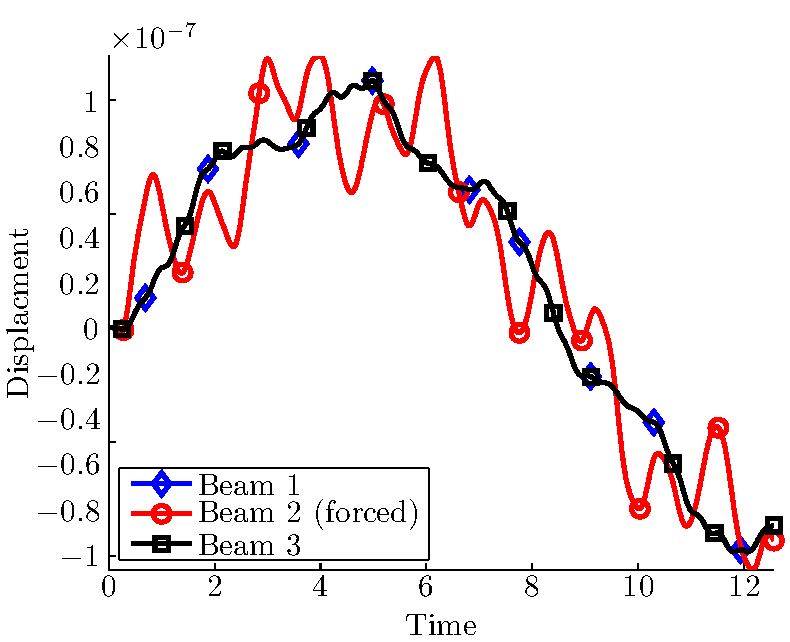
\includegraphics[width=0.75\textwidth]{images/w_forced_small_beta.pdf}
\end{figure}
\end{center}

\chapter{CONCLUSION}
\label{ch:conclusion}
\section{Summary of Work}
This thesis develops a finite element model for rotating cantilever beams from first physical principles. The energy equations are derived and variational calculus is applied to minimize the action functional. The test and weighting functions are derived and are the Hermite polynomials. These results are combined to create the discretized model. Finally, simulations are run to examine the system response to harmonic forcing.

Chapter two introduces the system in Cartesian coordinates.  The energy equations are then built using the Cartesian coordinate frame. A coordinate transformation produces a new hybrid coordinate frame with a stretch coordinate which describes elongation of the beam along its central axis. Elongation is described by the arclength integral so that the stretch coordinate $s$ is coupled to in-plane displacements $v$ and out-of-plane displacements $w$. The hybrid coordinate frame is substituted into the energy equations, then variational calculus is applied to the system to minimize the action functional, which produces the Euler-Lagrange equations. 

The test functions for the variational minimization are produced by considering the interpolating polynomials for the system. Enforcing boundary conditions on the interpolatory polynomials generates the Hermite polynomials. Thus, the test functions are the Hermite polynomials, which satisfy the requirements for application of variational minimization. Since the system is nonhomogeneous, Rayleigh-Ritz minimization no longer satisfies the minimization. Weighting functions are multiplied on the final result and then the system is minimized. The weighting functions are chosen to be the same as the test functions, thus Ritz-Galerkin is employed. Since the test and weight functions are the same and Hermite polynomials satisfy the conditions of both test and weight functions, the result of the minimization is the optimized form.

The discretization process breaks the beam into many coupled smaller beams. In order for the test and weight functions to be suitable for the minimization of the discretized beam, there must be continuity along the coupling. The Hermite polynomials provide this continuity, so the final form of the single-element beam optimization is acceptable for the coupled multi-element beam. The resulting matrix form  of the elemental Euler-Lagrange system are presented for easy application. Finally, the assembly process is described.

Chapter three presents the eigenvalue analysis of the produced system. The values are consistent with previous studies, thus the system is considered to be representative of the physical model. A f response analysis study is developed and the results show that harmonic forcing produces amplification of the natural modes. Then, forcing is applied to the system and the effects of periodic forcing as well as asymmetric forcing in the beam coupling terms are studied.

This work produced a descriptive manual for generating finite element models that represent physical systems with good agreement to previous work. Additionally, an application was developed in C++ that can easily be modified to both add terms for the Euler-Lagrange equations so that nonlinear analysis can be investigated, as well as adding stress-strain analysis. Furthermore, the routines written in MatLab provide eigenvalue and frequency response analysis capabilities that are also easy to modify according to changes in the model. Thus, this research provides a frame work for continued studies of coupled rotating cantilever beams.

\section{Further Work}
This study can be furthered in many ways. For one, the system can be modified to be a Timosheko beam system so that pretwisted beams can be studied. Additionally, a sweep over the coupling strength parameter $\beta$ would illuminate the importance of damping at the hub and more sophisticated models can be used to couple the beams around the hub. It would be beneficial to perform a MEX compilation of the C++ code so that the matrices that are assembled in the C++ code may be directly accessed by MatLab and not written to disk by C++ and read from the disk by MatLab. Furthermore, it would be useful to convert the algorithms presented here so that they can be used as a package add-on to a commercial off the shelf solver such as ANSYS or FEMAP/NASTRAN.

The fact that the trapezoid rule is the most accurate second order method and is A-stable presents the natural desire to utilize this method for the time integration. The fact that it is not L-stable presents issues with negative eigenvalues, as they will tend to result in oscillations in the solution. However, with a bit of effort, it is possible to develop integrators that are L-stable. Specifically, the implicit Runga-Kutta Radau I-A and Radau II-A schemes are L-stable and are third order accurate for the two step method. The increase of the number of steps (from one to two) is offset by the fact that there are no oscillations \emph{and} the the method converges with third order accuracy. While it was convenient to use MatLab's \texttt{ode23t} routine for this work, it would be natural to explore an implicit RK scheme to improve the efficiency of the integrator.
 
Finally, some of the linearity assumptions can be discarded to study nonlinear effects of the rotation and coupling. The linearity assumptions are tabulated in Appendix~\ref{app:assump}. Of the assumptions, the terms involving $\Omega$ are particularly interesting as their importance increases with increased rotation speed. To begin with, the assumption that the nonlinear bending coupling terms
\[\rho A\frac{\partial}{\partial x}\left\{\left[\int_L^x\Omega^2u\right]v_x\right\}\rightarrow 0\text{~~and~~}\rho A\frac{\partial}{\partial x}\left\{\left[\int_L^x\Omega^2u\right]w_x\right\}\rightarrow 0\]
should be discarded so that the presence of nonlinearities at high rotation speeds $\Omega$ in the coupling of $u$ to $v$- and $w$-bending can be studied. Since these terms depend on $\Omega^2$, it is clear that fast rotation speeds should increase the effects of these terms. Thus, it would be worthwhile to investigate this system with those terms included.